
\section{Ensamblaje final del sistema mecánico}

Se obtuvo una estructura integrada, con dimensiones de 47x52x57 cm y un peso general de 7.2kg.  Dicha plataforma sirvió como base de prueba para el sistema de extrusión diseñado que posteriormente se integró dando como resultado al sistema mecánico completo que cumple el propósito de impresión 3D totalmente funcional capaz de utilizar materiales PLA, TPU y PETG.
\subsection{Características obtenidas}
 
\begin{figure}[H]
    \centering
    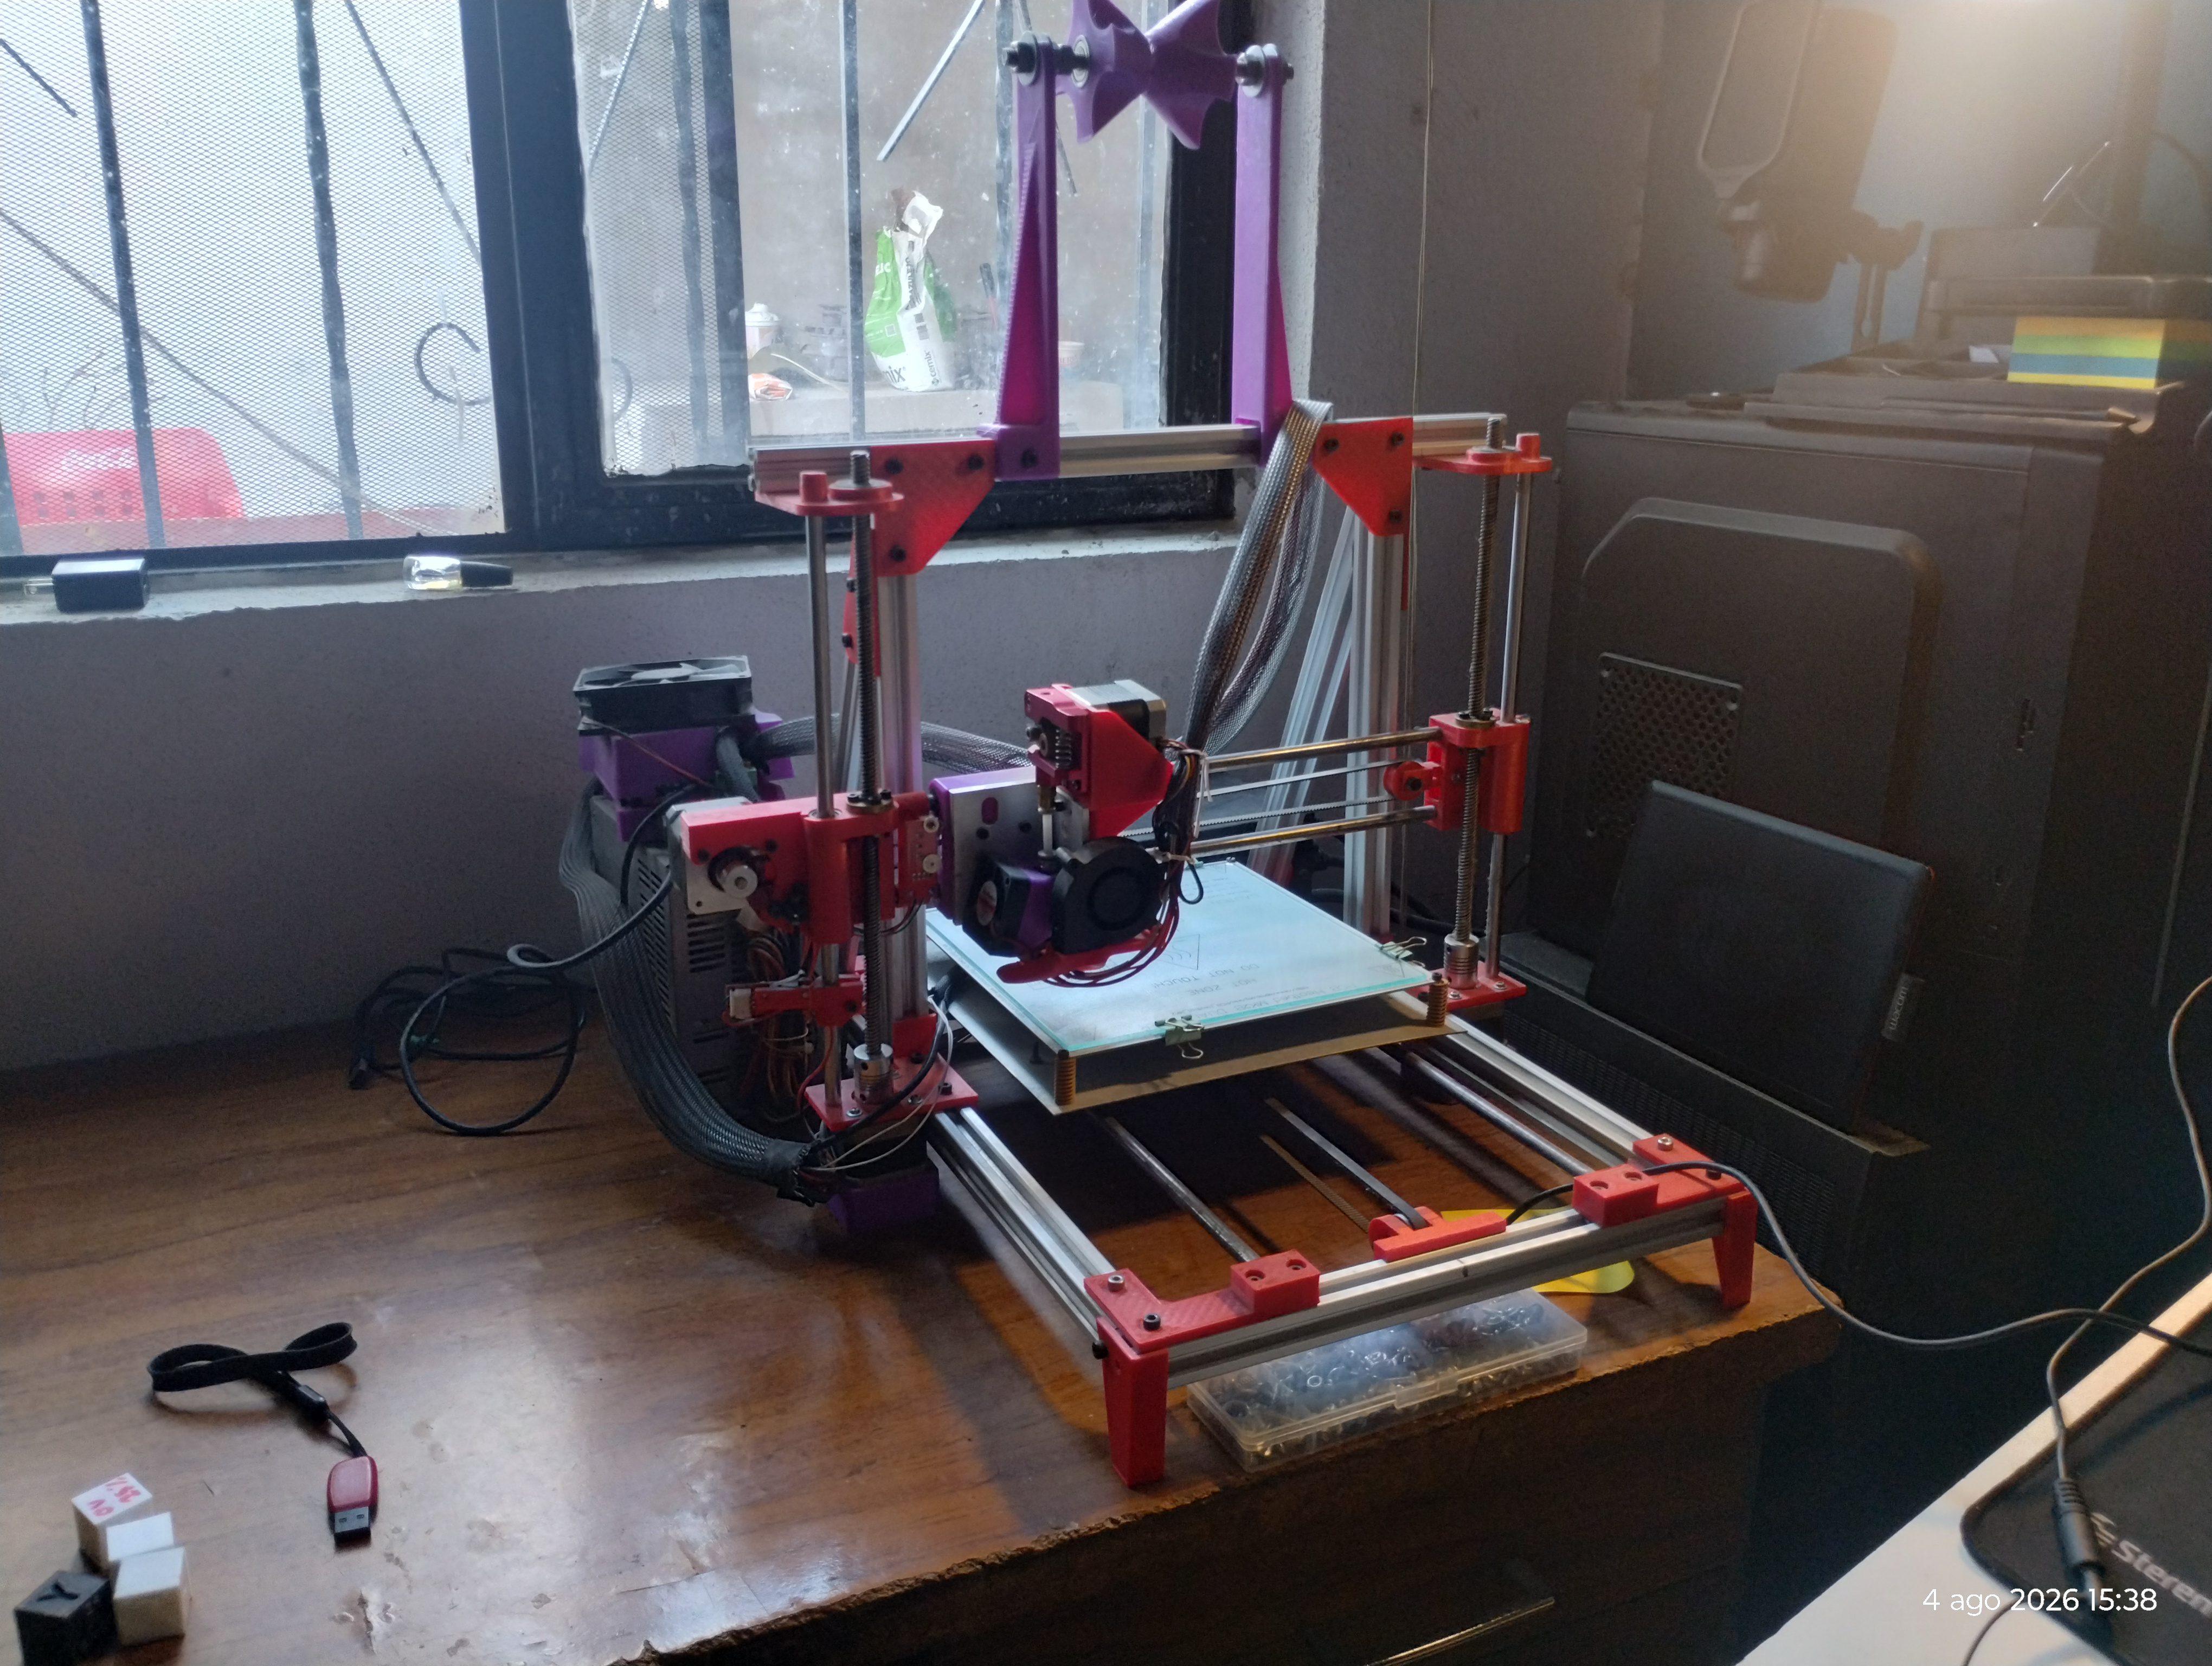
\includegraphics[width=0.5\linewidth]{Ensamblaje final.jpg}
    \caption{Ensamblaje final}
    \label{fig:placeholder111}
\end{figure}


\begin{comment}
\subsection{Estructura principal}
La estructura principal obtenida cumple con la rigidez necesaria para montar sobre de ella los tres ejes, donde a su vez van montados los distintos módulos: cama de impresión (eje Y), soporte del deslizante horizontal (eje Z) y soporte del extrusor (eje X). En este diseño no se contempló una base para soportar la fuente de alimentación por lo que esta suelta, lo cual podría ser una mejora a futuro. 

\subsection{Ejes}

\subsubsection{Eje Y}
El eje Y, encargado de mover la cama de impresión le debe su rigidez a la estructura principal ya que la varilla lisa se fijó directamente al perfil de aluminio (añadir que se hizo uso de otros diseños para los soportes de los rodamientos y la banda). La cama quedo montada sobre una lamina de acero galvanizado de calibre tal, suspendida por amortiguadores helicoidales  y en contacto directo con un vidrio templado fijado con grapas con el propósito de mejorar la superficie de impresión y aislamiento.

\subsubsection{Eje Z}
Al igual que el mencionado eje Y, el eje Z esta fijado directamente a la estructura principal dotándola de su rigidez y sus motores posados en el suelo directamente le otorgan a un mas firmeza al momento de la operacional del sistema. Este eje es el único de los tres en poseer varilla roscada para garantizar la fuerza necesaria para alzara al eje X que esta directamente montado sobre este.

\subsubsection{Eje X}

Montado sobre el eje Z, el eje X esta flotando sobre la cama de impresión y gracias a la rigidez del mencionado eje Z puede desplazarse sin comprometer su fuerza. Al igual que el eje Y, este tiene la capacidad de desplazarse por correas, obteniendo así un eje mas rápido en operación
\end{comment}

\subsection{Componentes adicionales}
\subsubsection{Finales de carrera}
Fuera del diseño elegido. Los soportes de los limites de carrera son importantes en el comportamiento del sistema completo, ya que otorga mayor repetitividad en los resultados al poder determinar un origen en la operación que el sistema va a realizar y con ello lograr una automatizaron del proceso.
\subsubsection{Case para controlador}
Con fines de organizar el cableado y  salvaguardar la integridad del controlador del sistema, se eligió un case  popular (dar creditos)

\subsubsection{Soporte carrete}
Aportando a la  comodidad a la hora del funcionamiento del sistema, se eligió el añadirle un soporte para el carrete de filamento. El cual obtiene su rigidez  directamente de la estructura principal.

\subsubsection{Reforzamiento estructural}
Los ángulos  le añaden aun mas rigidez a la estructura principal y cumplen satisfactoriamente su función. Obteniendo asi una base aun mas solida para todos los componentes.



\begin{comment}
Contenido:

Fotografía del ensamble completo.
Render del modelo CAD final.
Descripción del marco:
dimensiones externas,
volumen ocupado,
área de impresión obtenida.
Peso aproximado del cabezal de impresión.

(una tabla comparativa)

Sistema mecánico ensamblado
Descripción del ensamble final: dimensiones del marco, área de impresión resultante, peso aproximado del cabezal.

(Mencionar que de las primeras mejoras del extrusor diseñado es que la altura del mismo es menor al que tiene el diseño)

\end{comment}

\section{Mejora del sistema de extrusión}
El sistema de extrusión obtenido tiene las dimensiones de 14 cm de alto por 10 cm de ancho y 7 cm de largo. Con un peso de 493 gramos.







\begin{figure}[H]
    \centering
    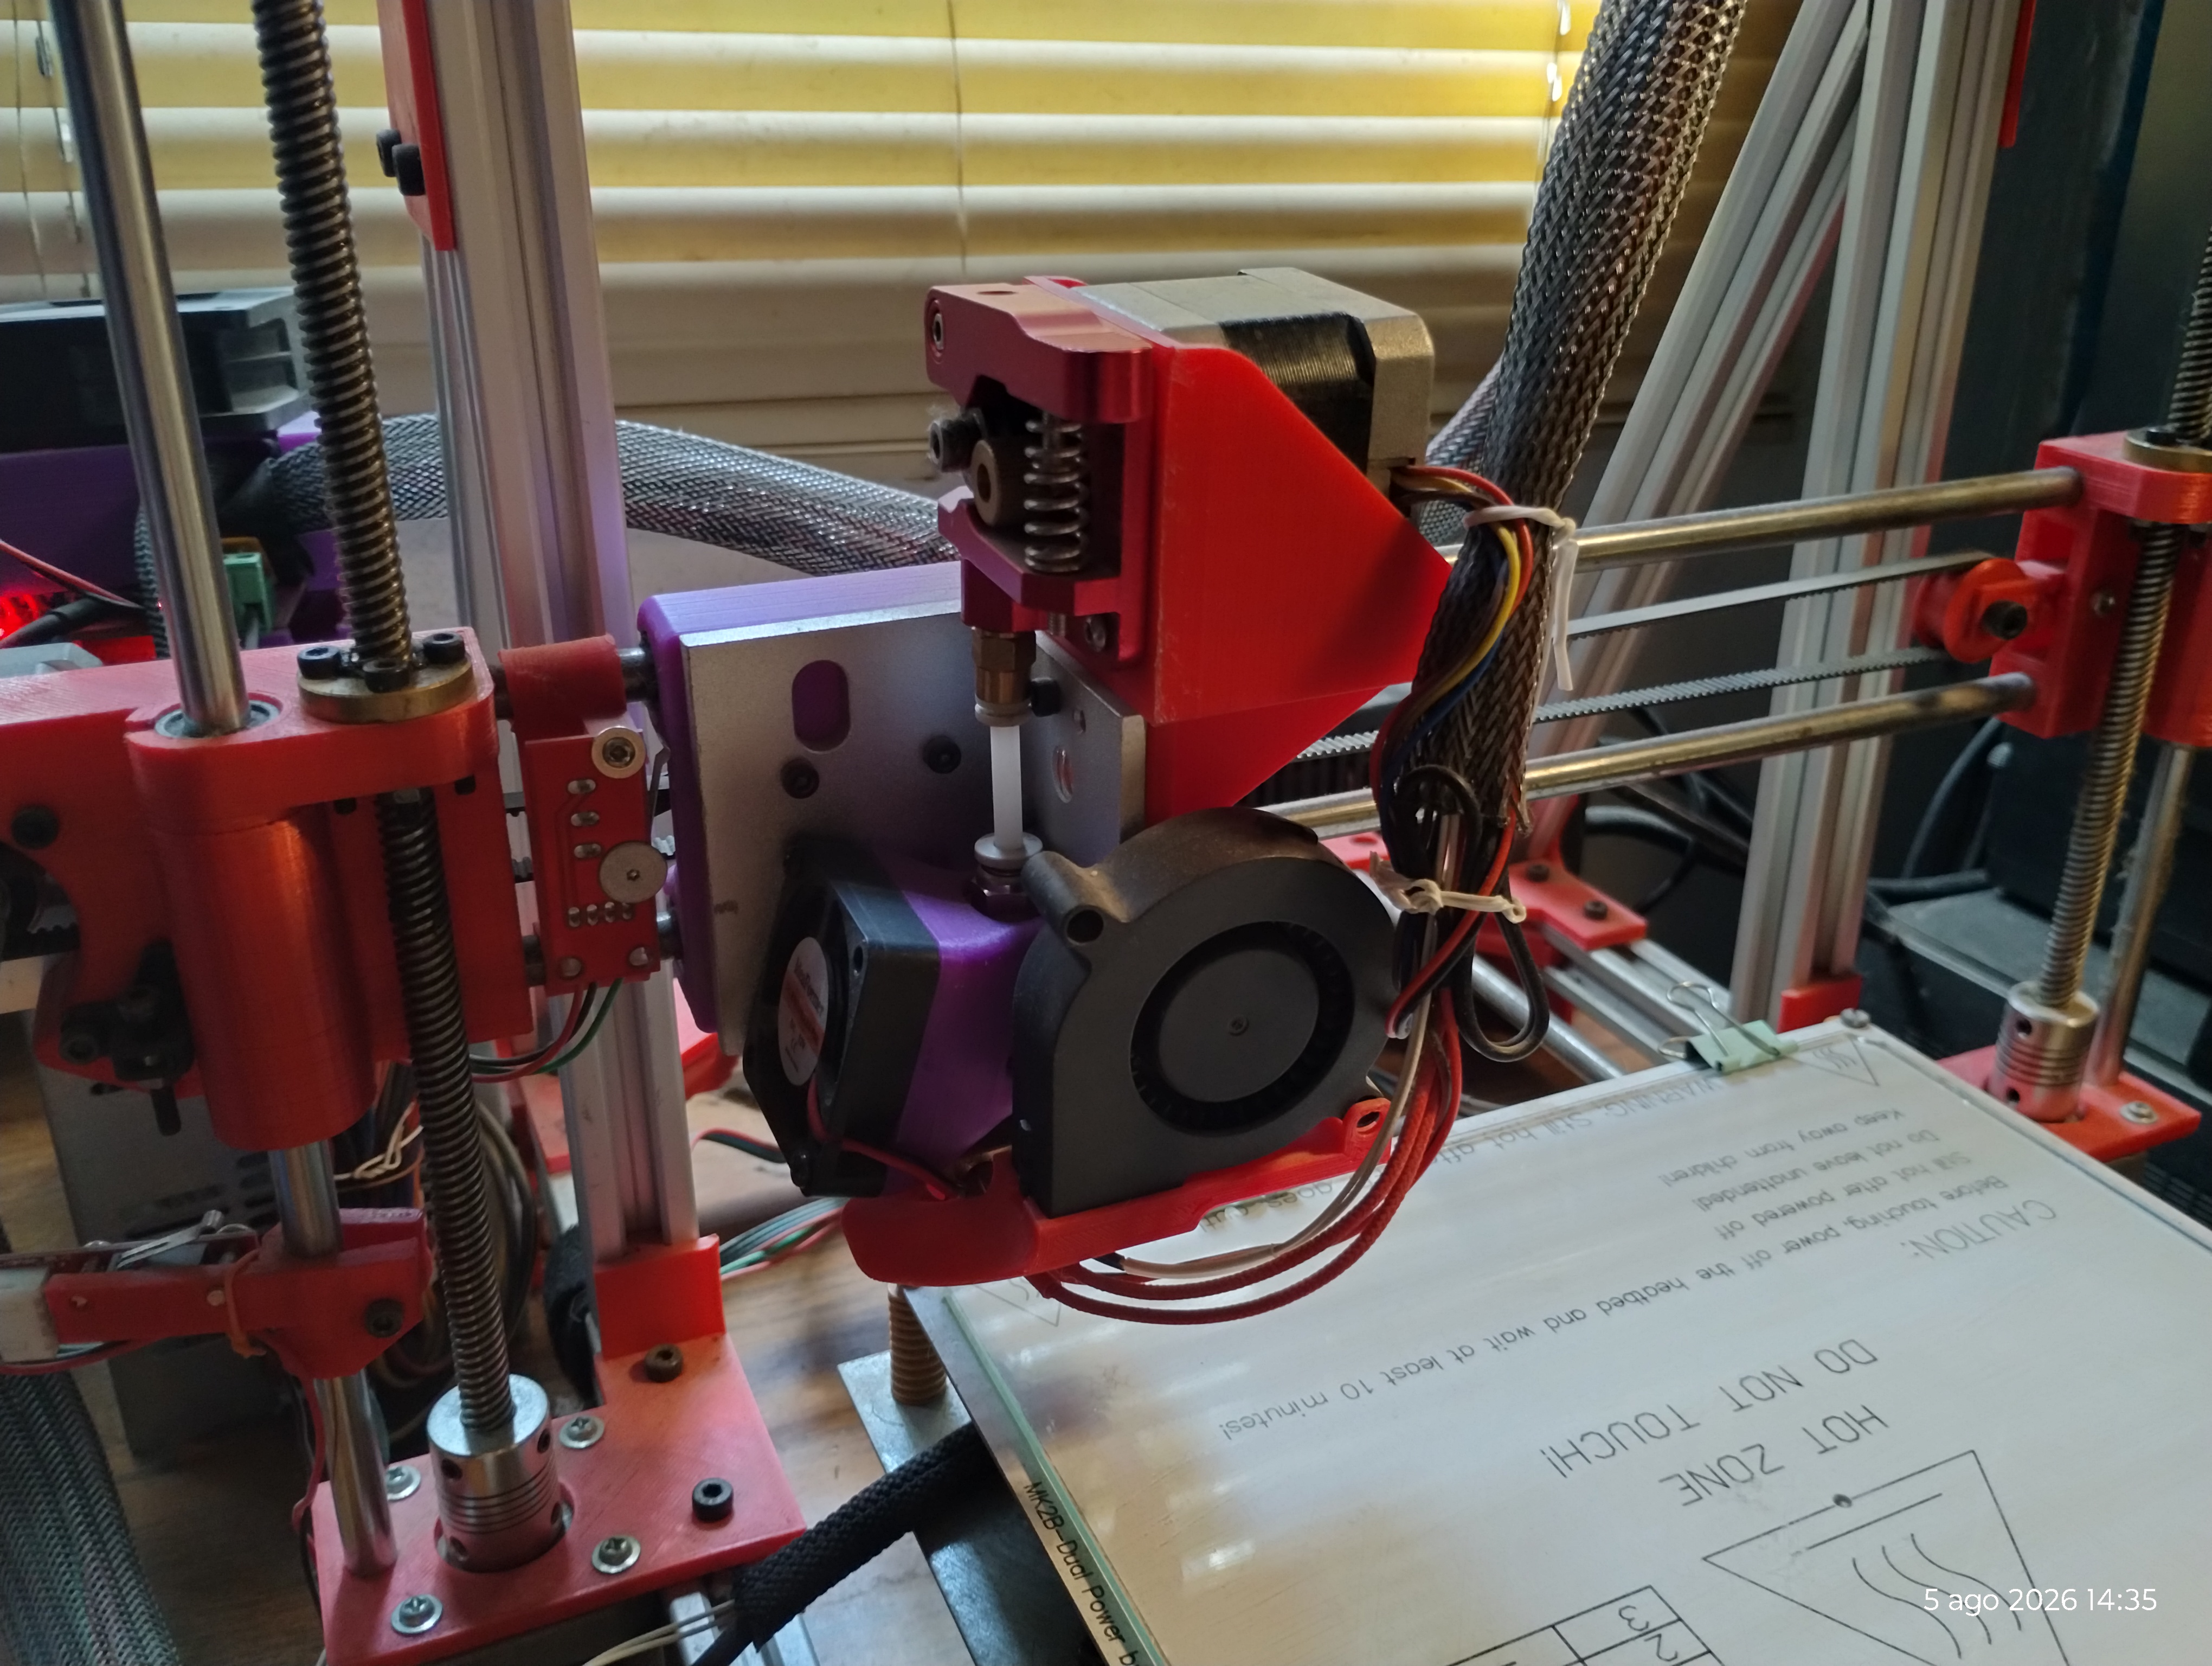
\includegraphics[width=0.5\linewidth]{Extrusor final.jpg}
    \caption{Extrusor final}
    \label{fig:placeholder222}
\end{figure}




\begin{comment}
    Descripción geométrica de la solución final: dimensiones clave, separación entre motor y hotend, geometría del sistema de ventilación.
(render SolidWorks o foto de la pieza, comparativa visual de los 3 intentos)

Comparación directa entre el diseño realizado con un diseño antiguo. 

Primera mejora considerable es la altura que ocupa el extrusor antiguo y el que ocupa el primero. 

Necesito imprimir cosas con el extrusor antiguo y el nuevo ( tomar foto de evidencia de la calidad de la impresión y de la altura que se ocupa para dicho extrusor.
\end{comment}

\section{Validación del funcionamiento}


\subsection{Sistema de movimiento}

\subsubsection{Moviomiento de los ejes X-Y}
provisional ....Se verificó el funcionamiento de los ejes X y Y mediante desplazamientos controlados desde el firmware. En todos los casos los ejes recorrieron la totalidad de su trayectoria sin presentar pérdidas de pasos, atascamientos ni vibraciones que comprometieran el movimiento. Asimismo, se comprobó la repetibilidad de los desplazamientos mediante movimientos sucesivos entre posiciones definidas, obteniéndose un comportamiento uniforme en los dos ejes.

\begin{figure}[H]
    \centering
    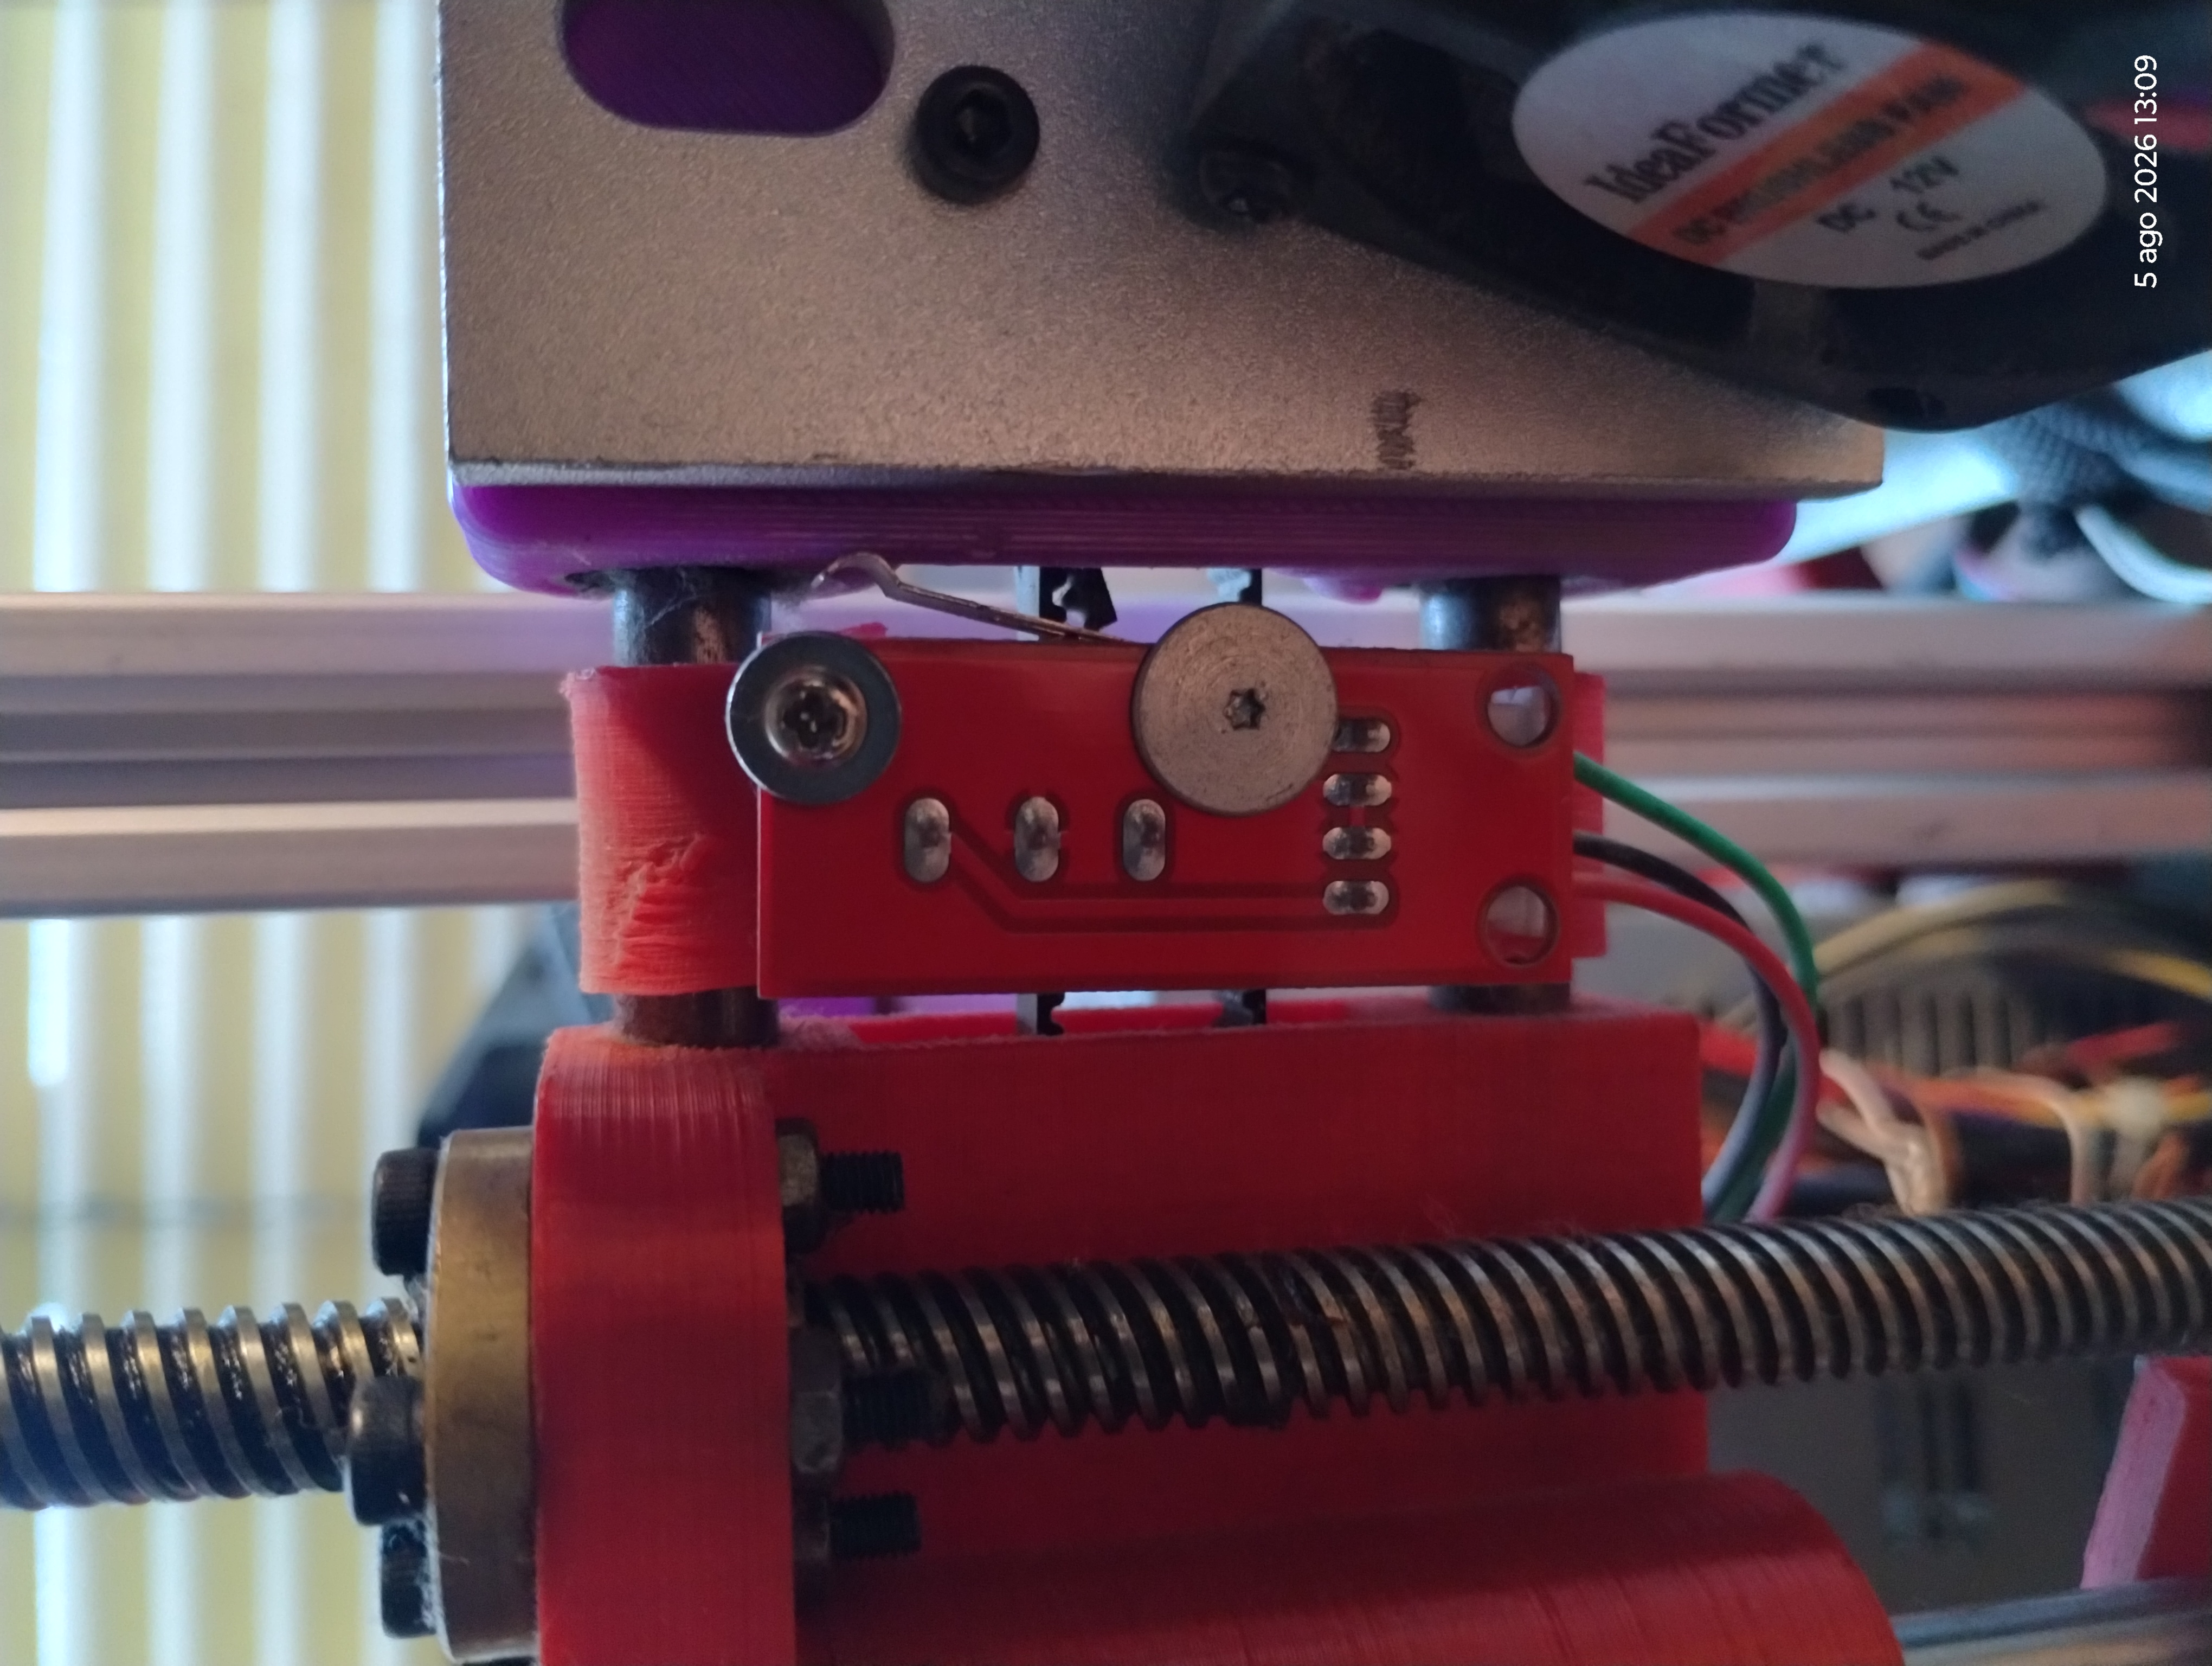
\includegraphics[width=0.5\linewidth]{limiteX.jpg}
    \caption{Evidencia de validacion demovimiento X-Y}
    \label{fig:placeholder333}
\end{figure}


\begin{table}[H]
\centering
\small
\caption{Validación del sistema de movimiento.}
\label{tab:validacion_movimiento}
\begin{tabular}{p{2cm} p{8cm} p{3cm}}
\toprule
\textbf{Eje} & \textbf{Prueba realizada} & \textbf{Resultado} \\
\midrule

X &
Desplazamiento completo del carro a lo largo del recorrido mediante comandos enviados desde el firmware, verificando ausencia de pérdidas de pasos y atascamientos. &
Correcto \\

\addlinespace

Y &
Desplazamiento completo de la cama de impresión, comprobando un movimiento uniforme y repetible durante recorridos sucesivos. &
Correcto \\

\addlinespace



\bottomrule
\end{tabular}
\end{table}
\subsubsection{Movimiento del eje Z}
 El caso del eje Z es distinto a los otros dos, gracias a que este obtiene su movimiento a dos husillos y tiene la función de cargar al eje X. Por lo cual su validación es
 distinta, al contar con dos motores que ejercen la fuerza para alzar el eje x, fue necesario comprobar el correcto desplazamiento ambos y determinar si existió o no una desviación. 
\begin{figure}[H]
    \centering
    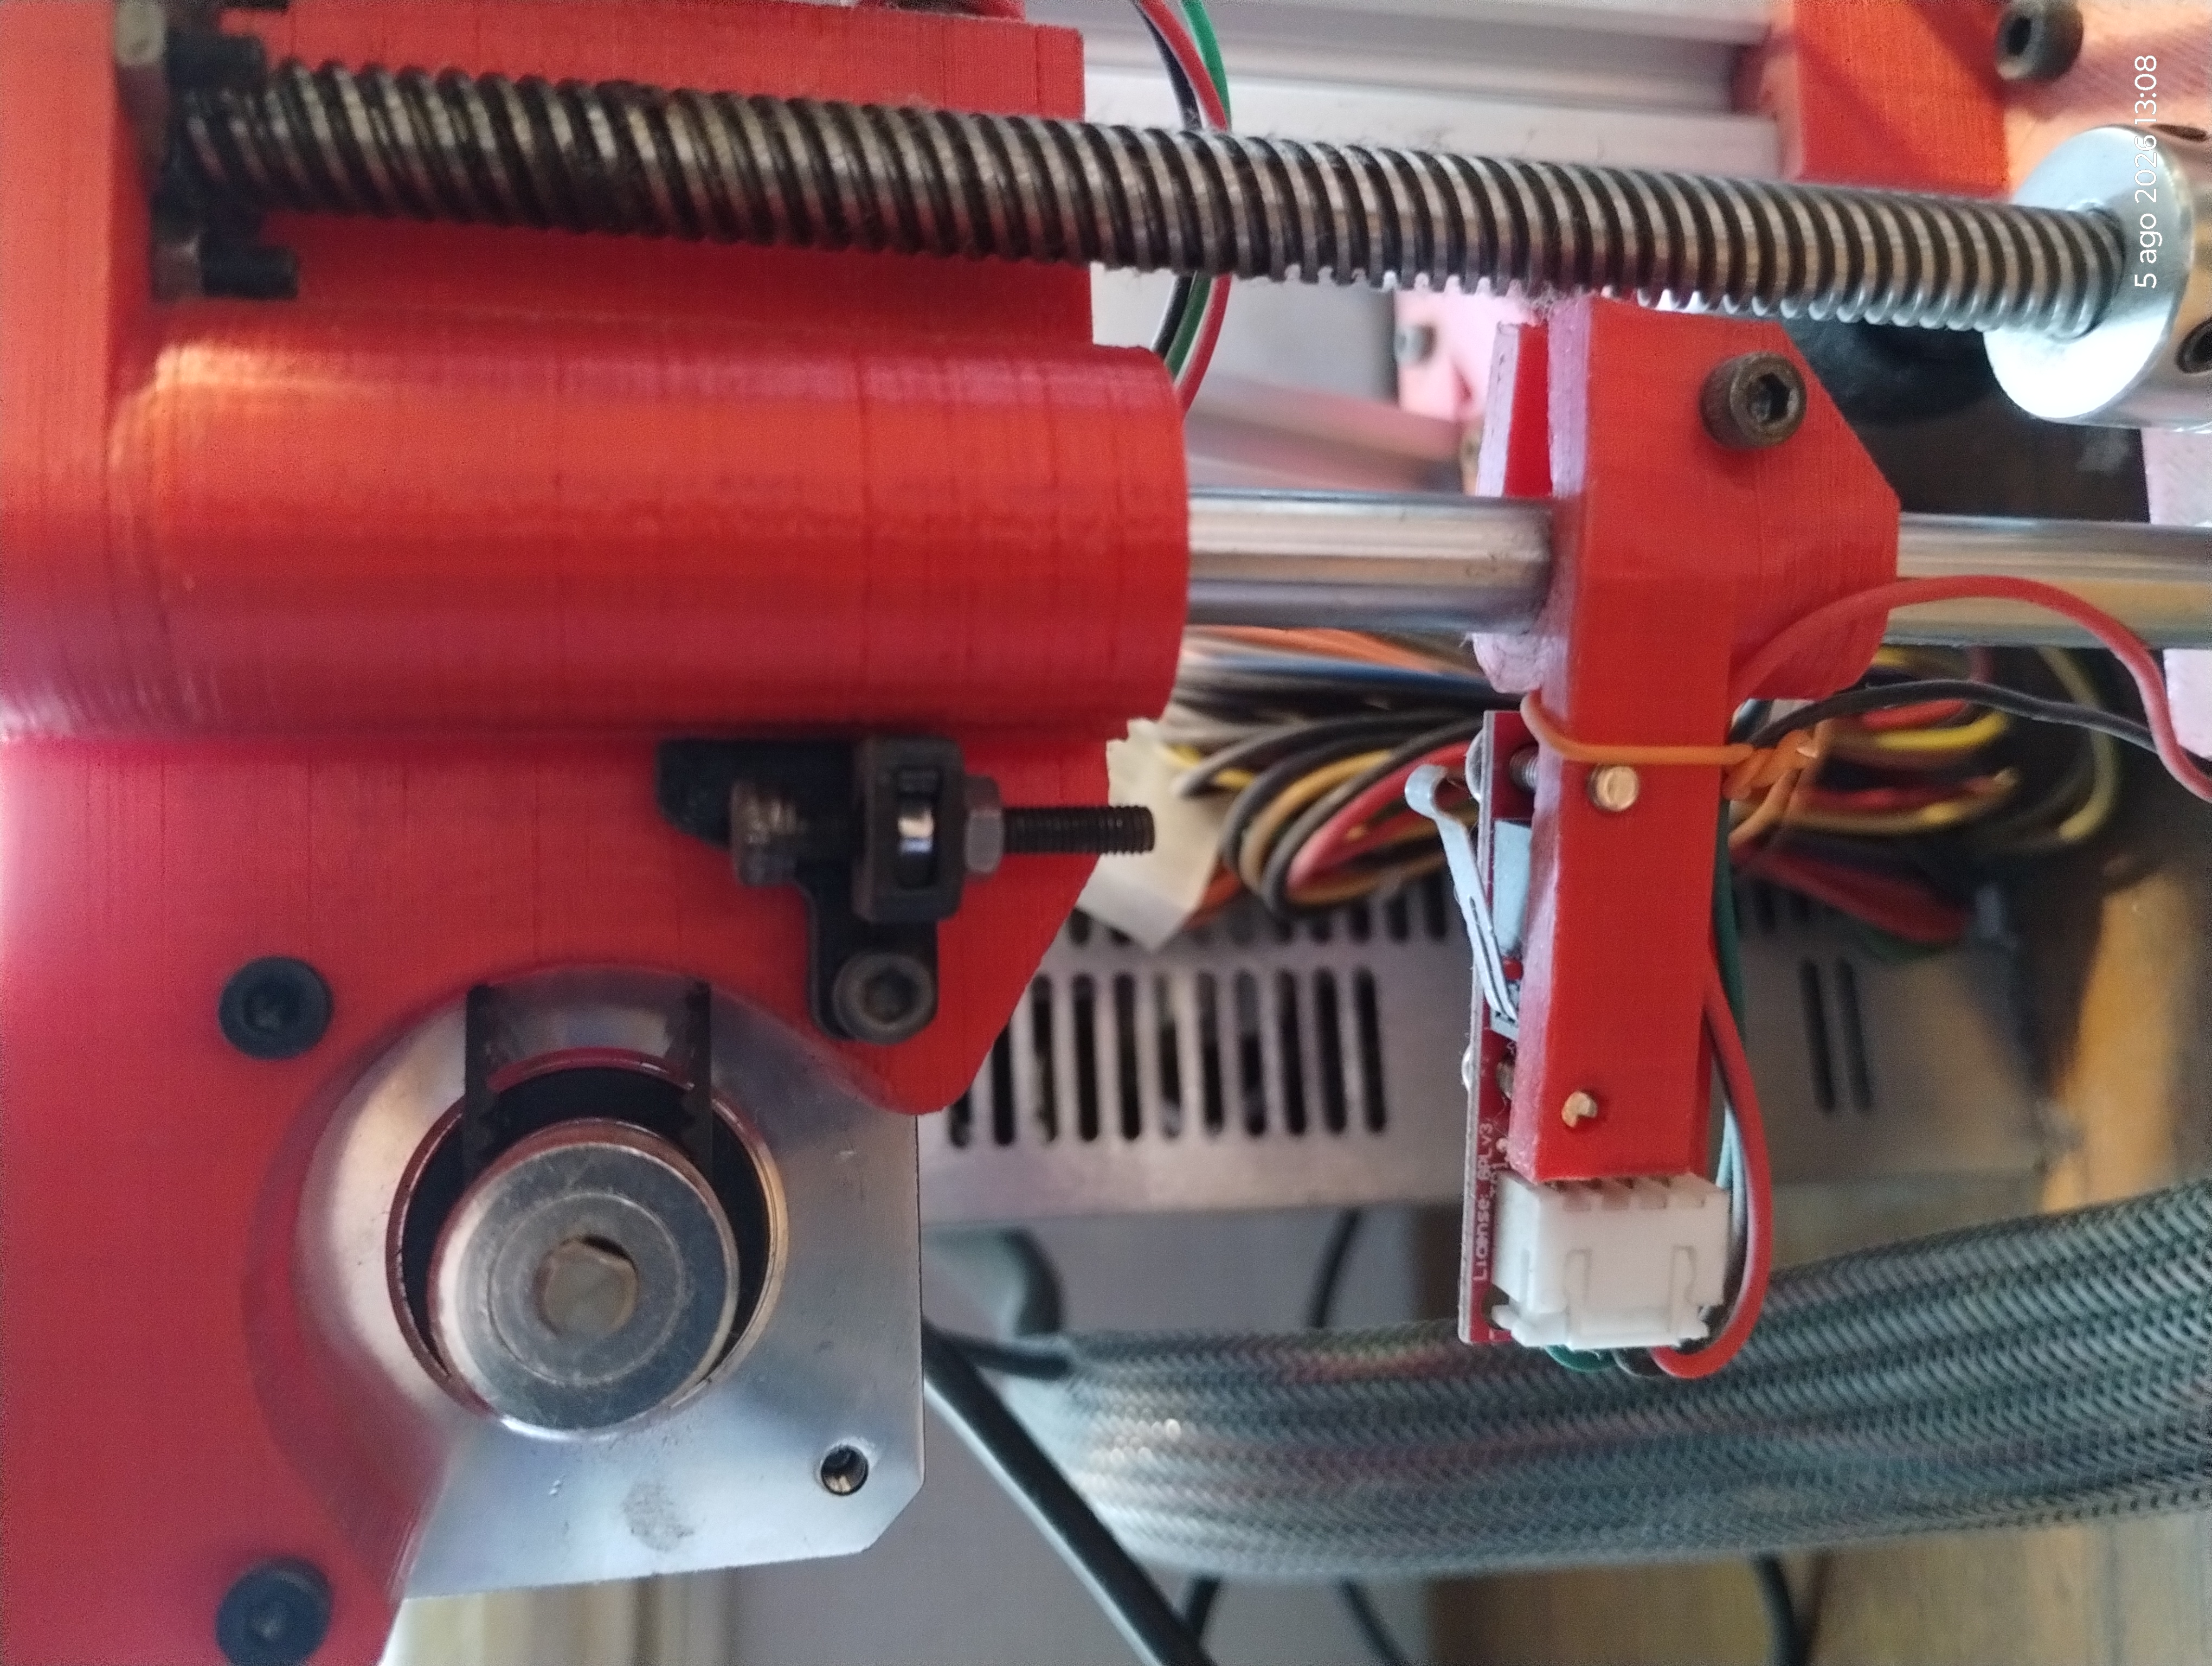
\includegraphics[width=0.5\linewidth]{calibrador altura de capa.jpg}
    \caption{Eje Z}
    \label{fig:placeholder444}
\end{figure}

 Despues de realizar la mediciones correspondientes, se obtuvo un comportamiento aceptable con un error menor al (porcentanje). Lo cual garantiza un funcionamiento confiable y repetible.


 
\subsubsection{Finales de carrera}


\begin{figure}[H]
    \centering
    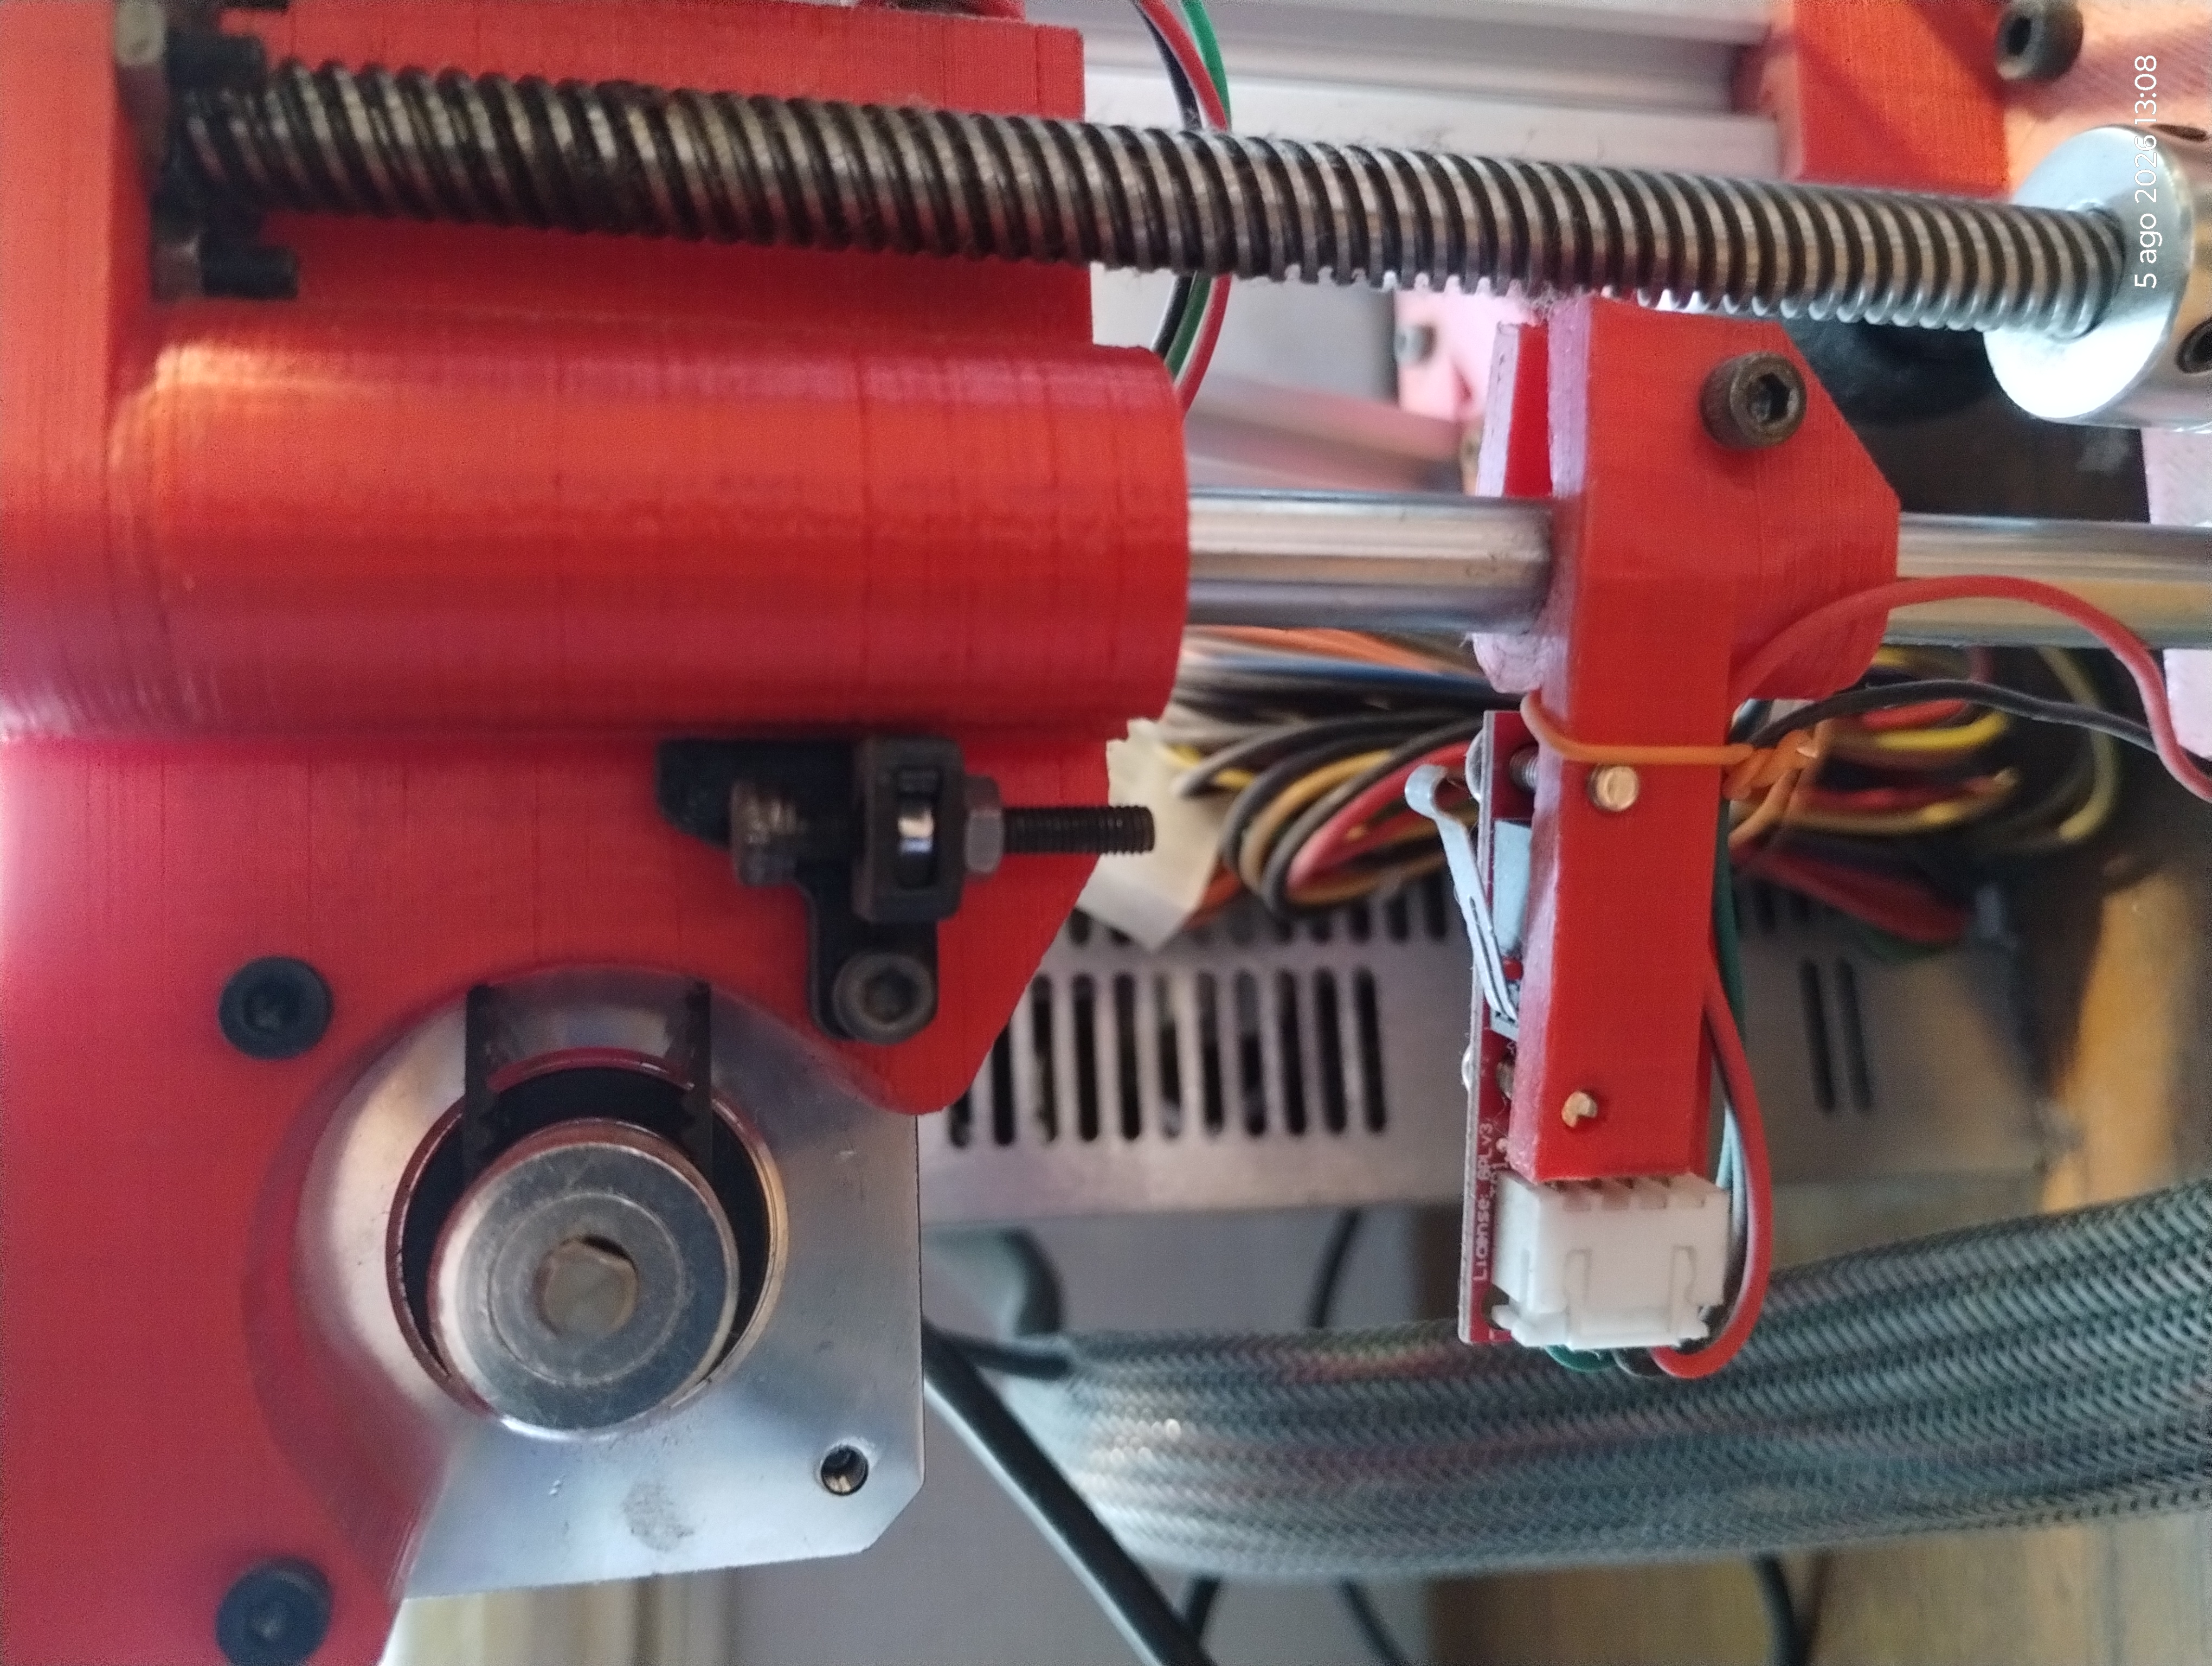
\includegraphics[width=0.5\linewidth]{calibrador altura de capa.jpg}
    \caption{Calibrador de altura de capa}
    \label{fig:placeholder555}
\end{figure}

\subsection{Sistema de extrusión}
temperatura máxima;
ausencia/presencia de deformación;
número de iteraciones;
etc.
\subsubsection{Hotend}
Al estar sujeto directamente al angulo de aluminio, el hotend tiene contacto directo con un metal con alta conductividad térmica y en conjunto con su ventilador, logra disipar gran cantidad de calor que de otra manera podría afectar al flujo correcto de filamento. Este diseño obtenido logro disipar el 12 por ciento de la temperatura alcanzada en el cabezal, lo cual significa una baja considerable y evita que el filamento se vea deformado antes de llegar al cabezal, lo cual ayuda a que el sistema no sufra atascos recurrentes.

\subsubsection{Extrusor mecánico}
La pieza impresa en PLA tiene una resistencia a la deformación mecánica de (). Al ser fabricada en una sola pieza de cuerpo unido, es capaz de resistir la fuerza de empuje que ejerce el motor sin presentar deformaciones. Debido a las capacidades anteriormente mencionadas, este diseño cumple con los requisitos mínimos para realizar un trabajo repetitivo sin tener la preocupación de que vaya a deformarse rápidamente.

---------Durante las pruebas de extrusión no se observaron deformaciones permanentes en la pieza impresa ni desplazamientos entre el motor y el mecanismo de alimentación.--------


\subsubsection{Enfriador de capa}
Este modulo siendo de gran importancia relacionado directamente con la calidad de impresión, llegando a distintas iteraciones para llegar a este resultado final que cumple satisfactoriamente el enfriamiento necesario y dimensiones aceptables. Pruebas de flujo?

---------una tabla con las diferentes iteraciones---------------

    \begin{figure}[H]
    \centering
    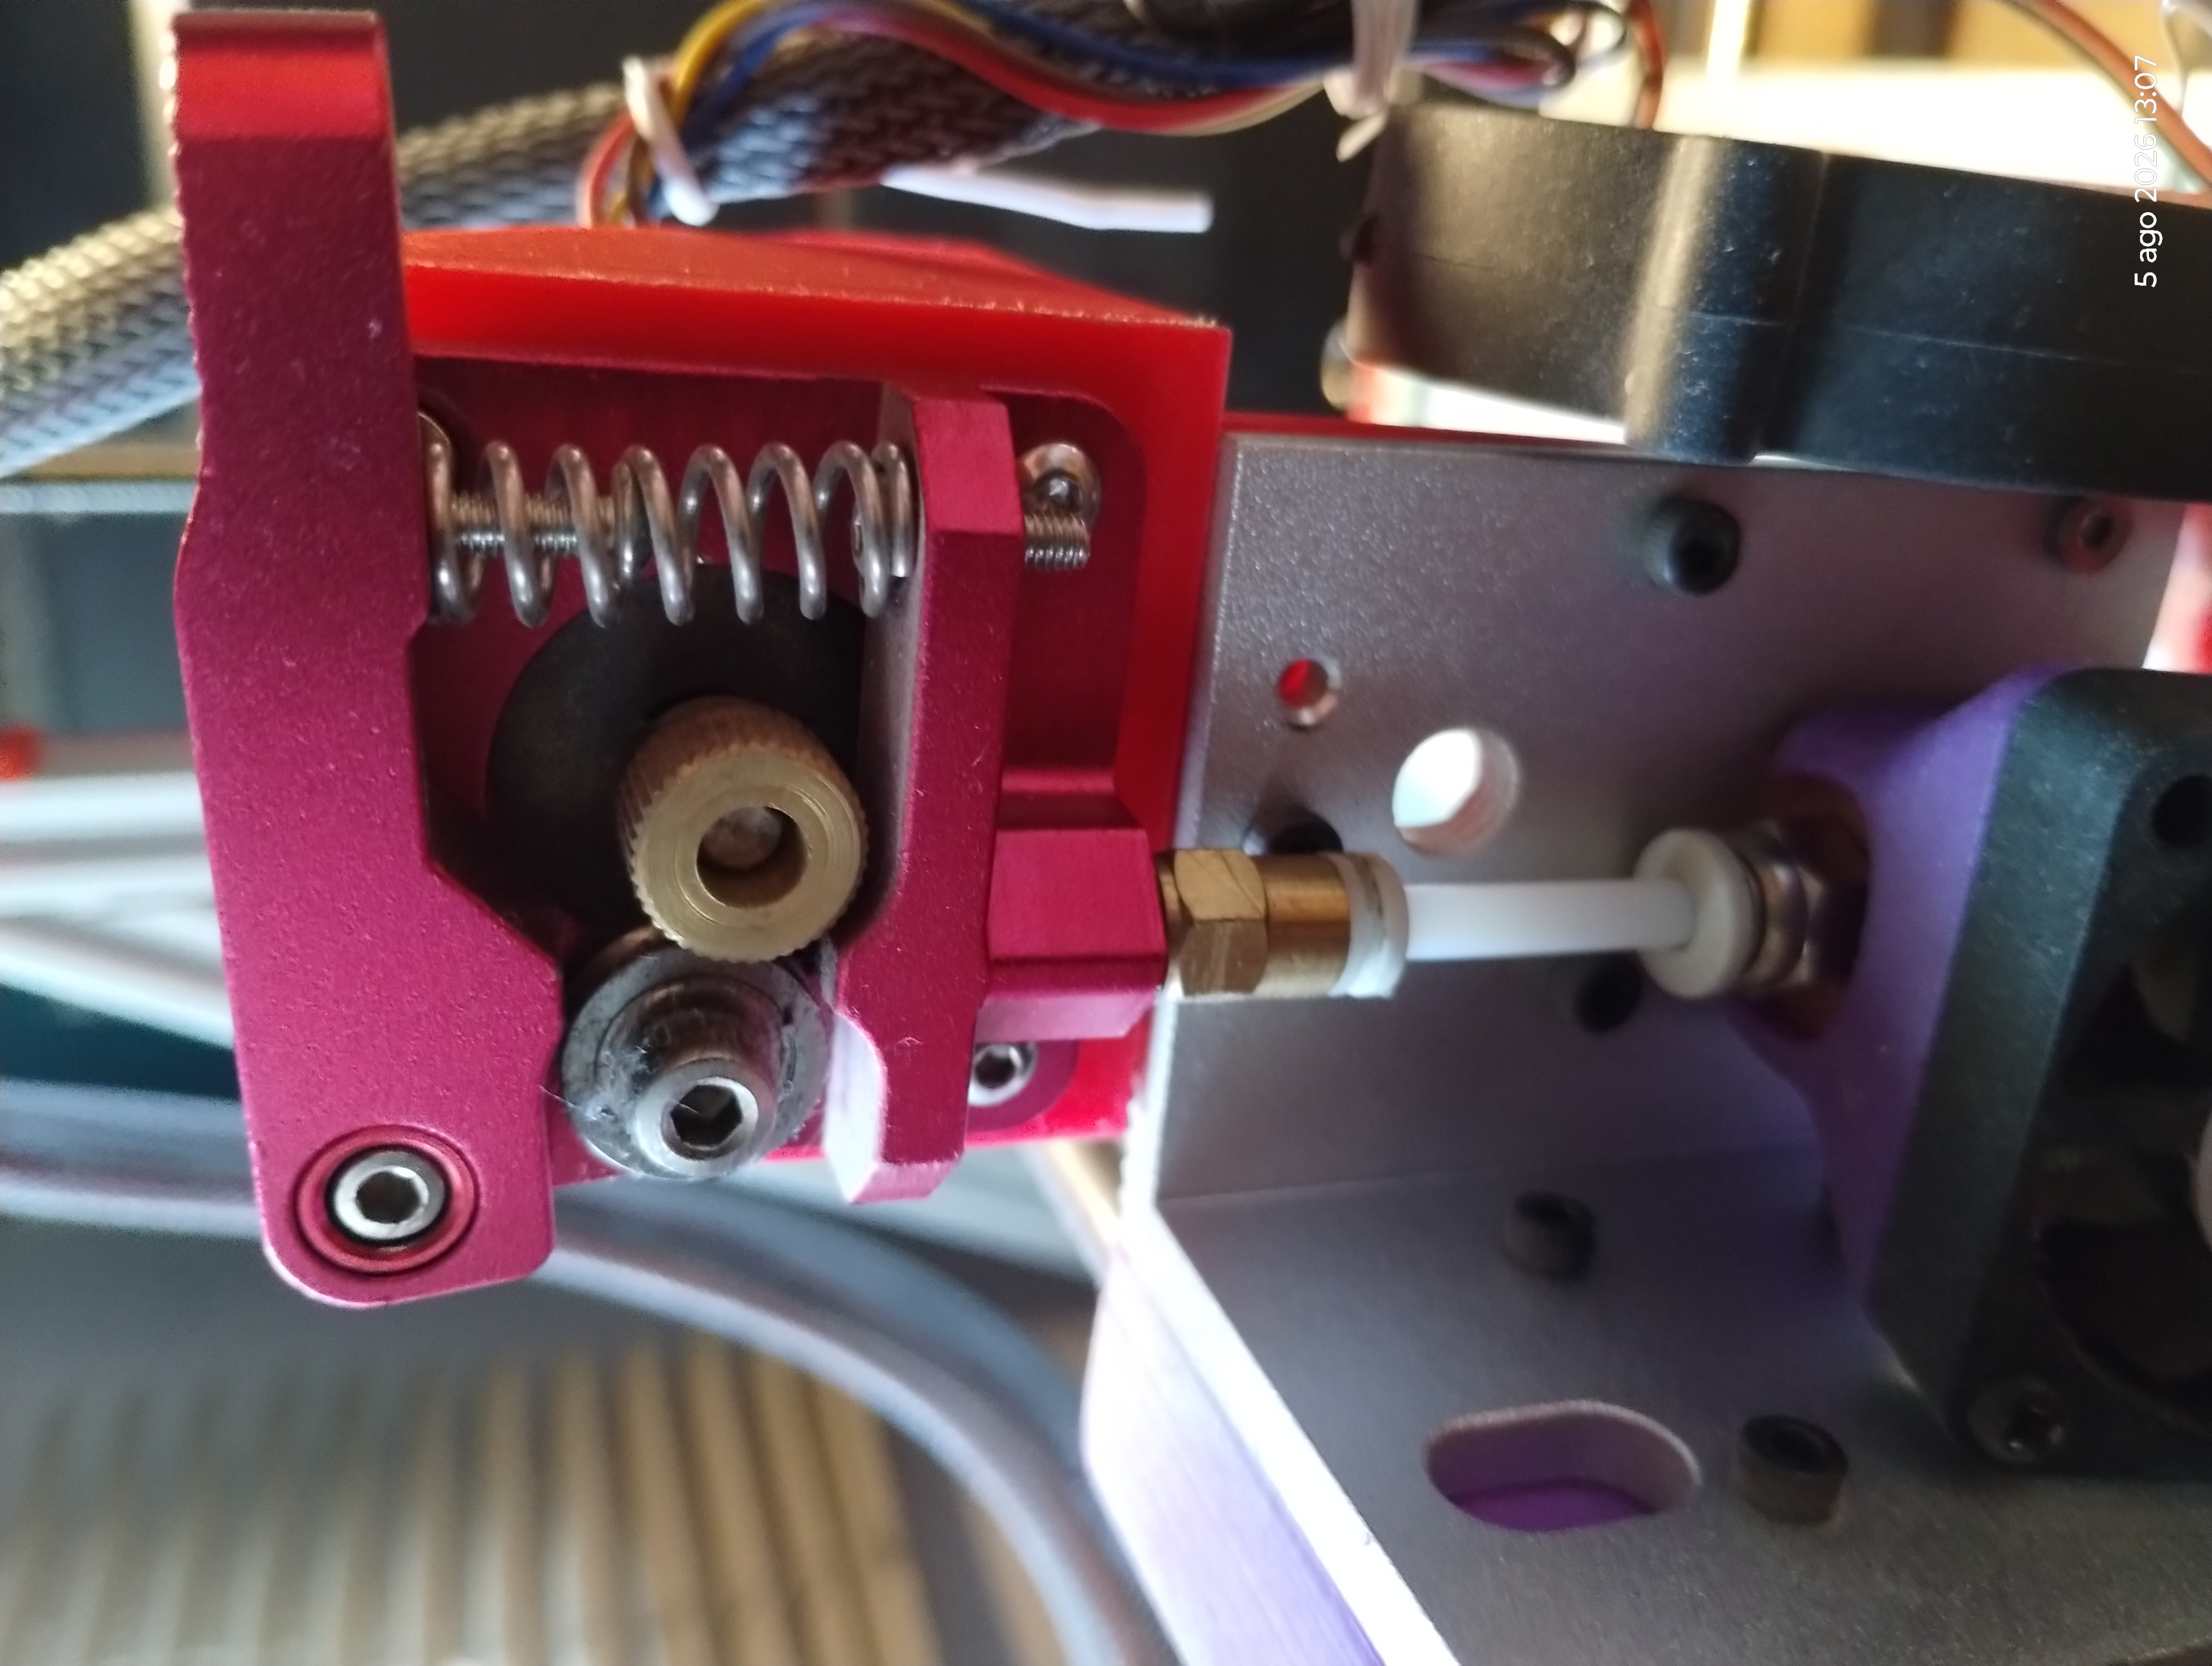
\includegraphics[width=0.5\linewidth]{Extrusor.jpg}
    \caption{Sistema de extrusión}
    \label{fig:placeholder656}
\end{figure}


Alimentación continua sin deslizamientos.
\subsection{Sistema de calentamiento}
\subsubsection{Hotend}

    \begin{figure}[H]
    \centering
    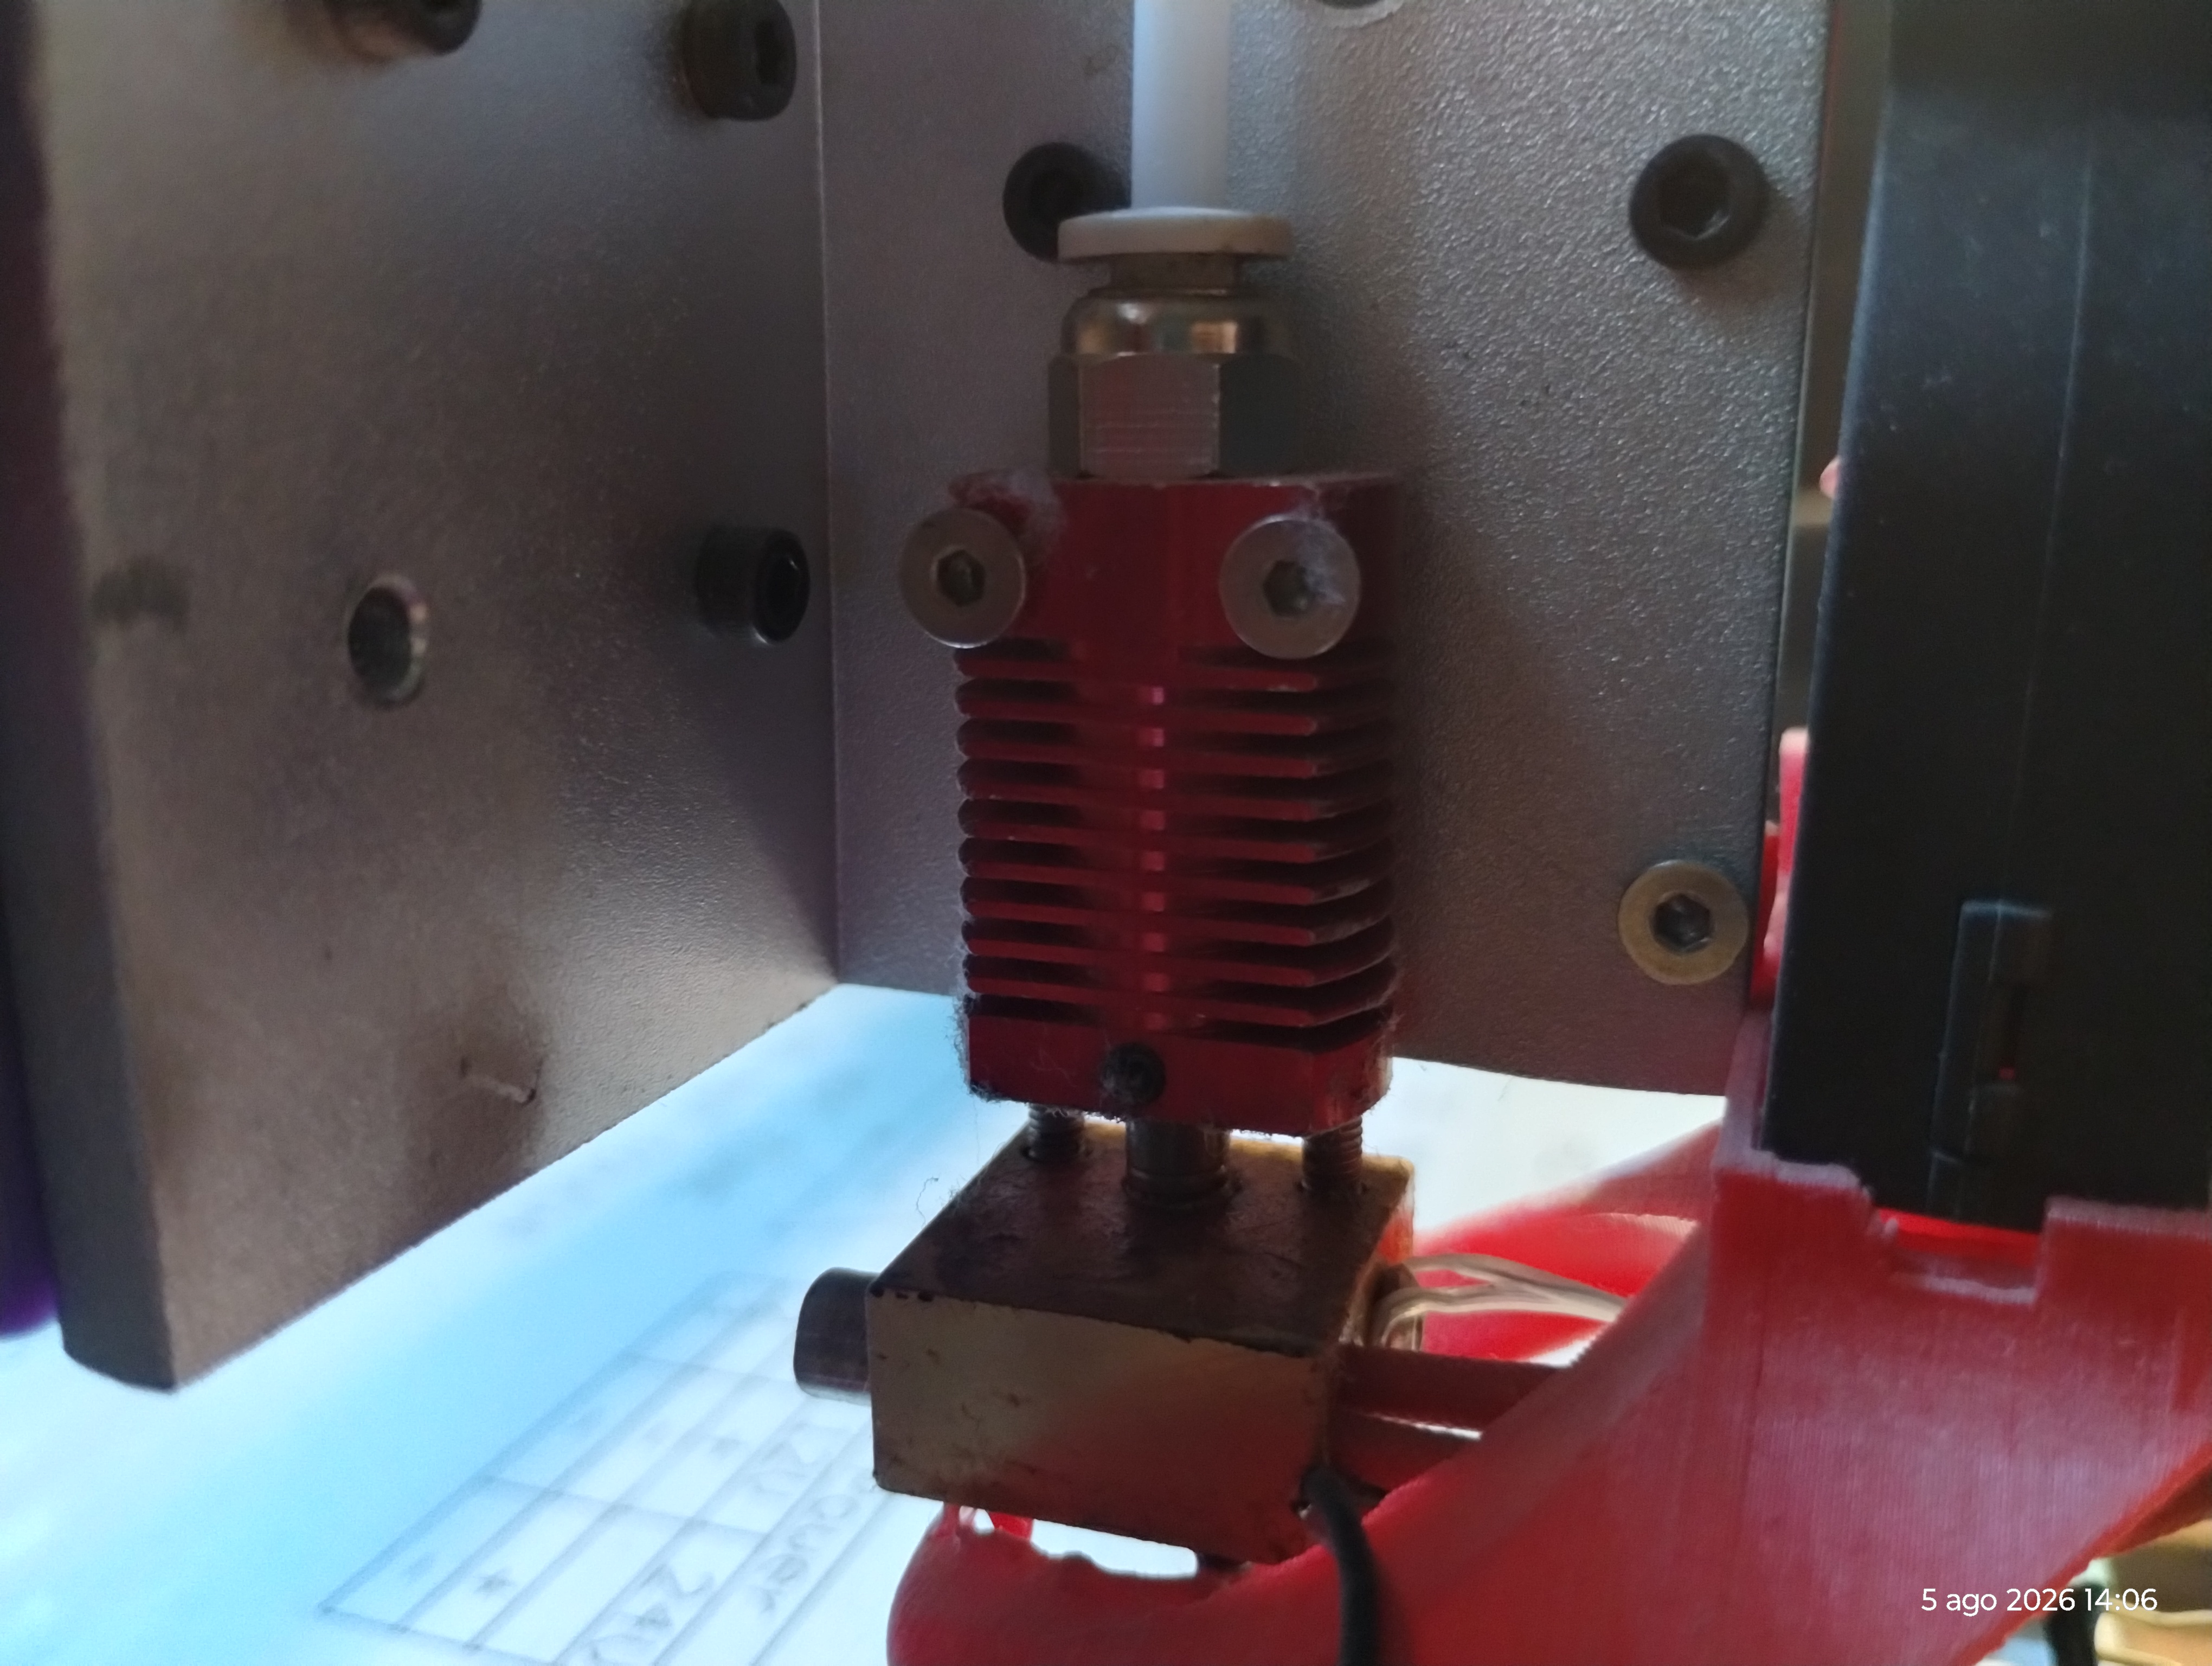
\includegraphics[width=0.5\linewidth]{hotend.jpg}
    \caption{Hotend}
    \label{fig:placeholder777}
\end{figure}





Alcanzó y mantuvo la temperatura programada.
\subsubsection{Cama caliente}

    
\begin{figure}[H]
    \centering
    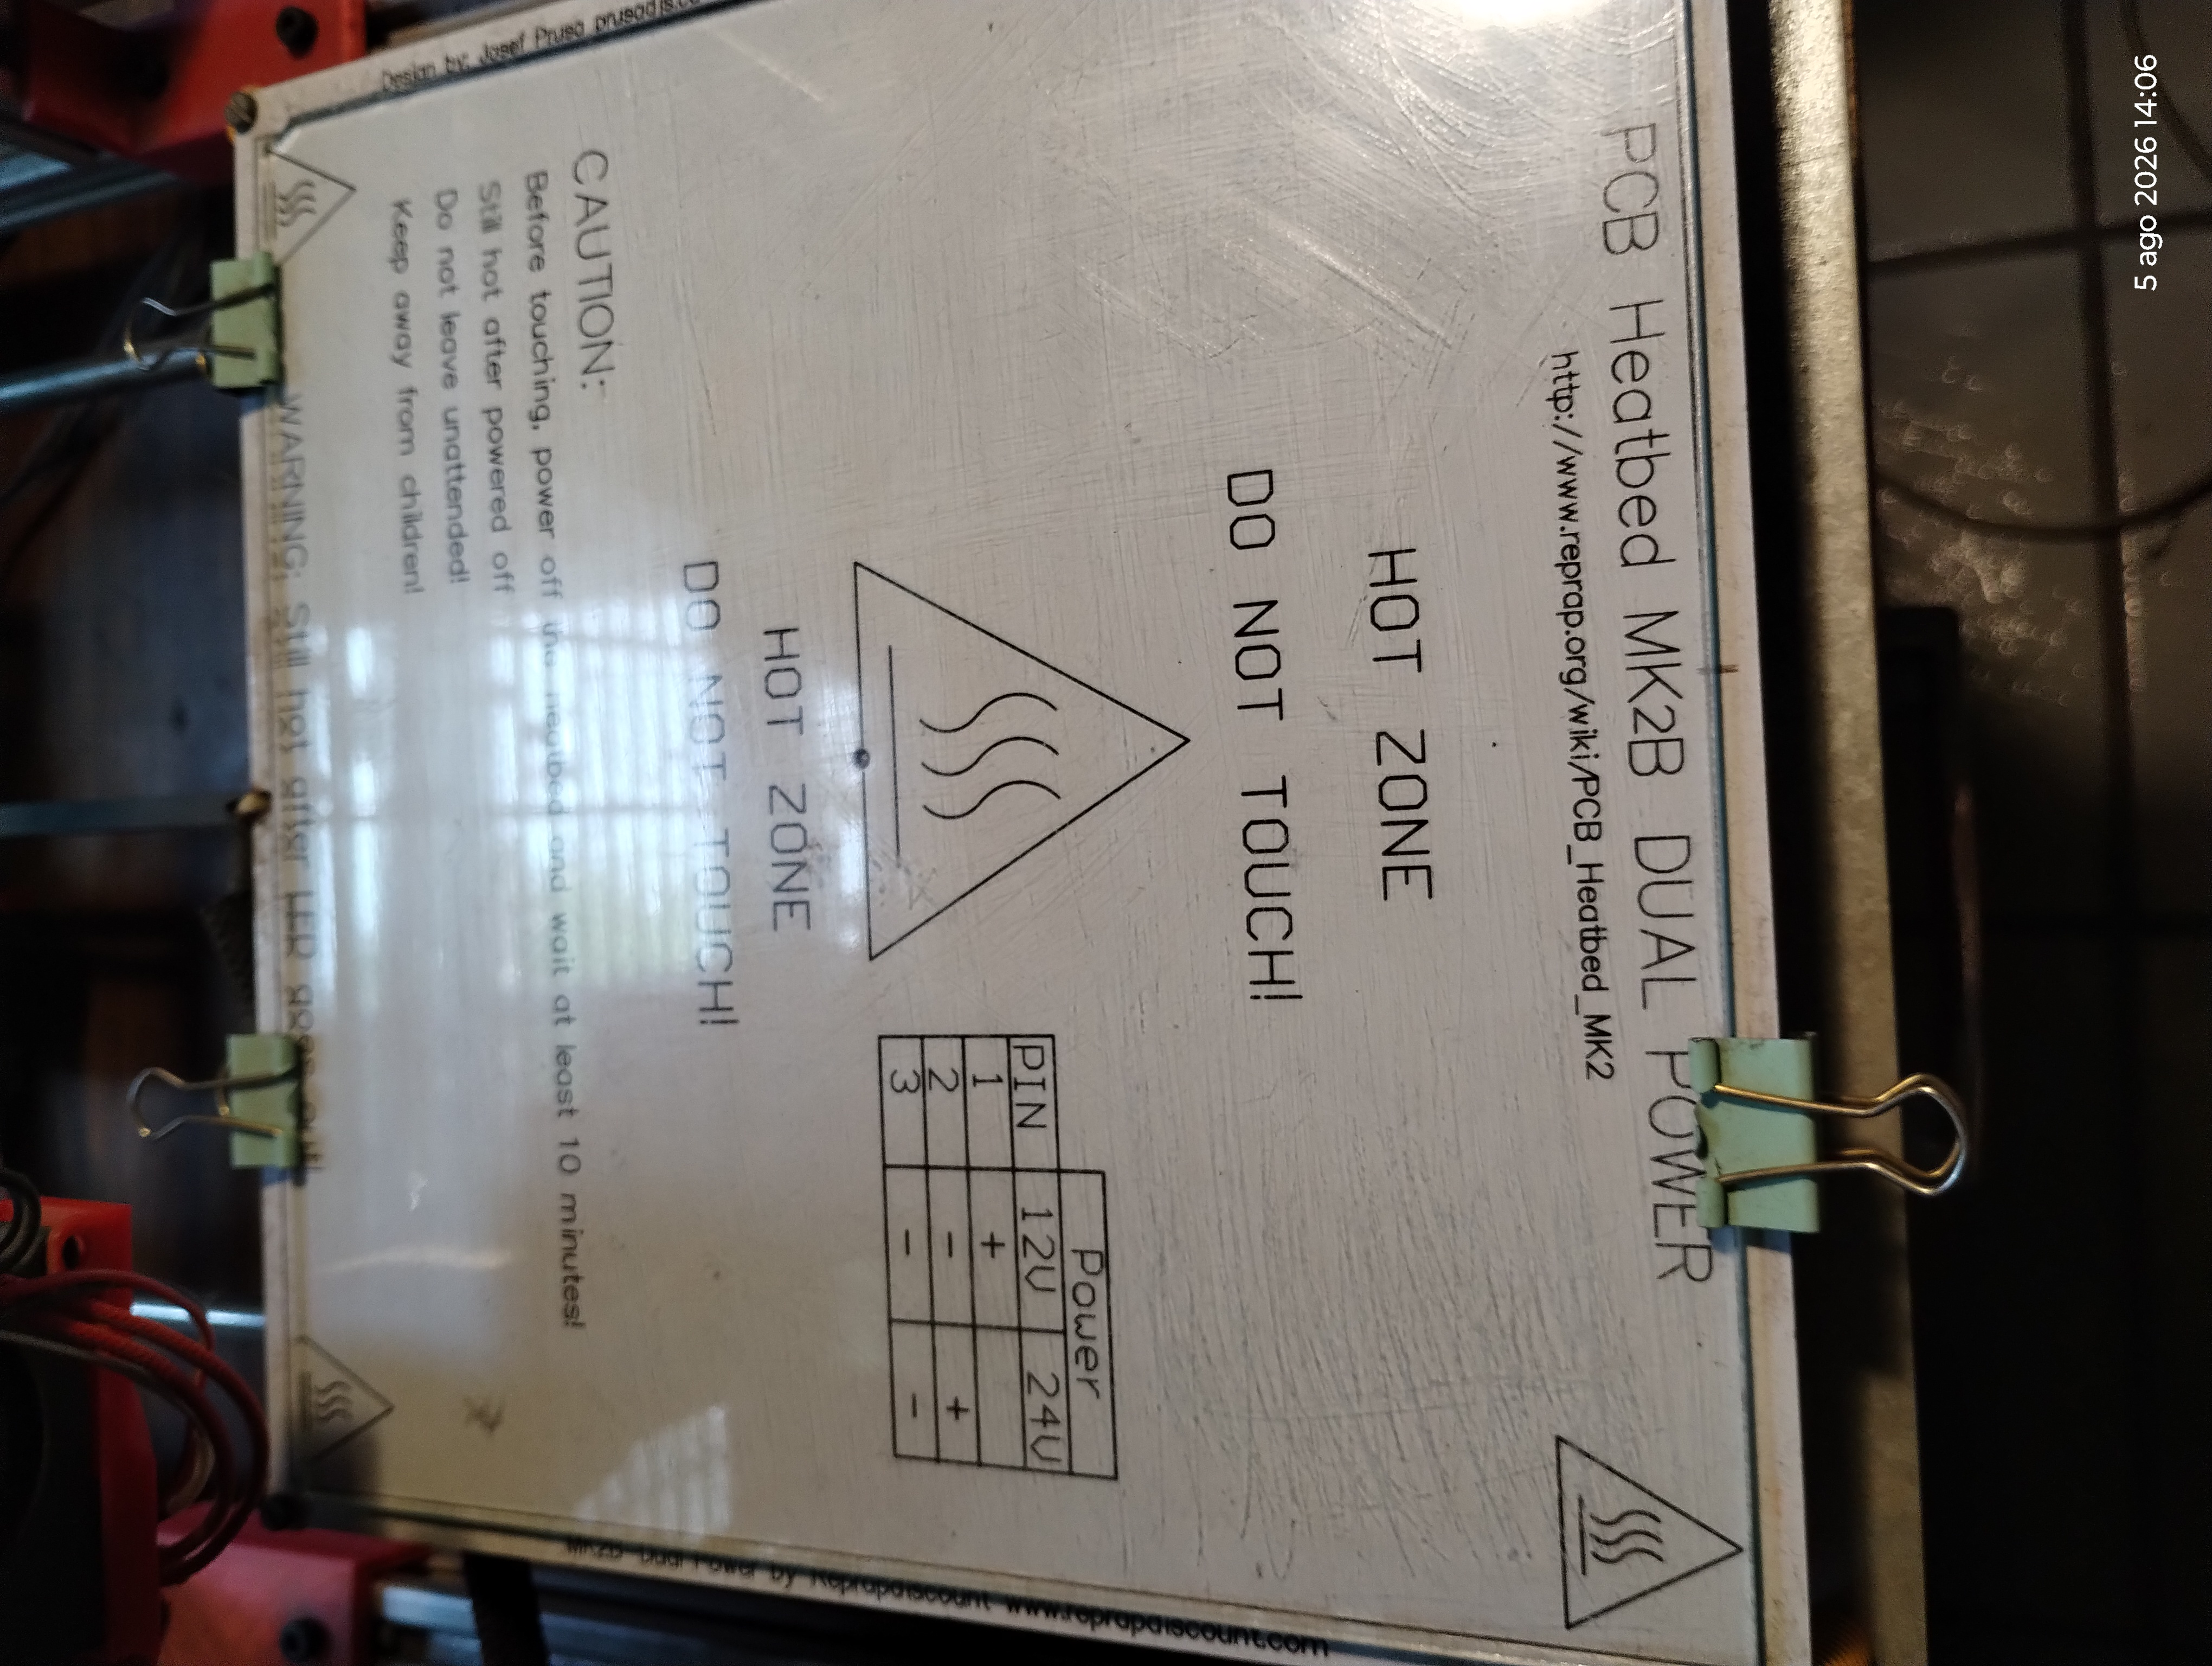
\includegraphics[width=0.5\linewidth]{cama de impresion.jpg}
    \caption{Cama caliente}
    \label{fig:placeholder888}
\end{figure}

 Tabla de temperaturas con y sin disipacion de hotend 

\
\
\
\
Alcanzó la temperatura configurada.
\subsubsection{Ventilación}

\begin{figure}[H]
    \centering
    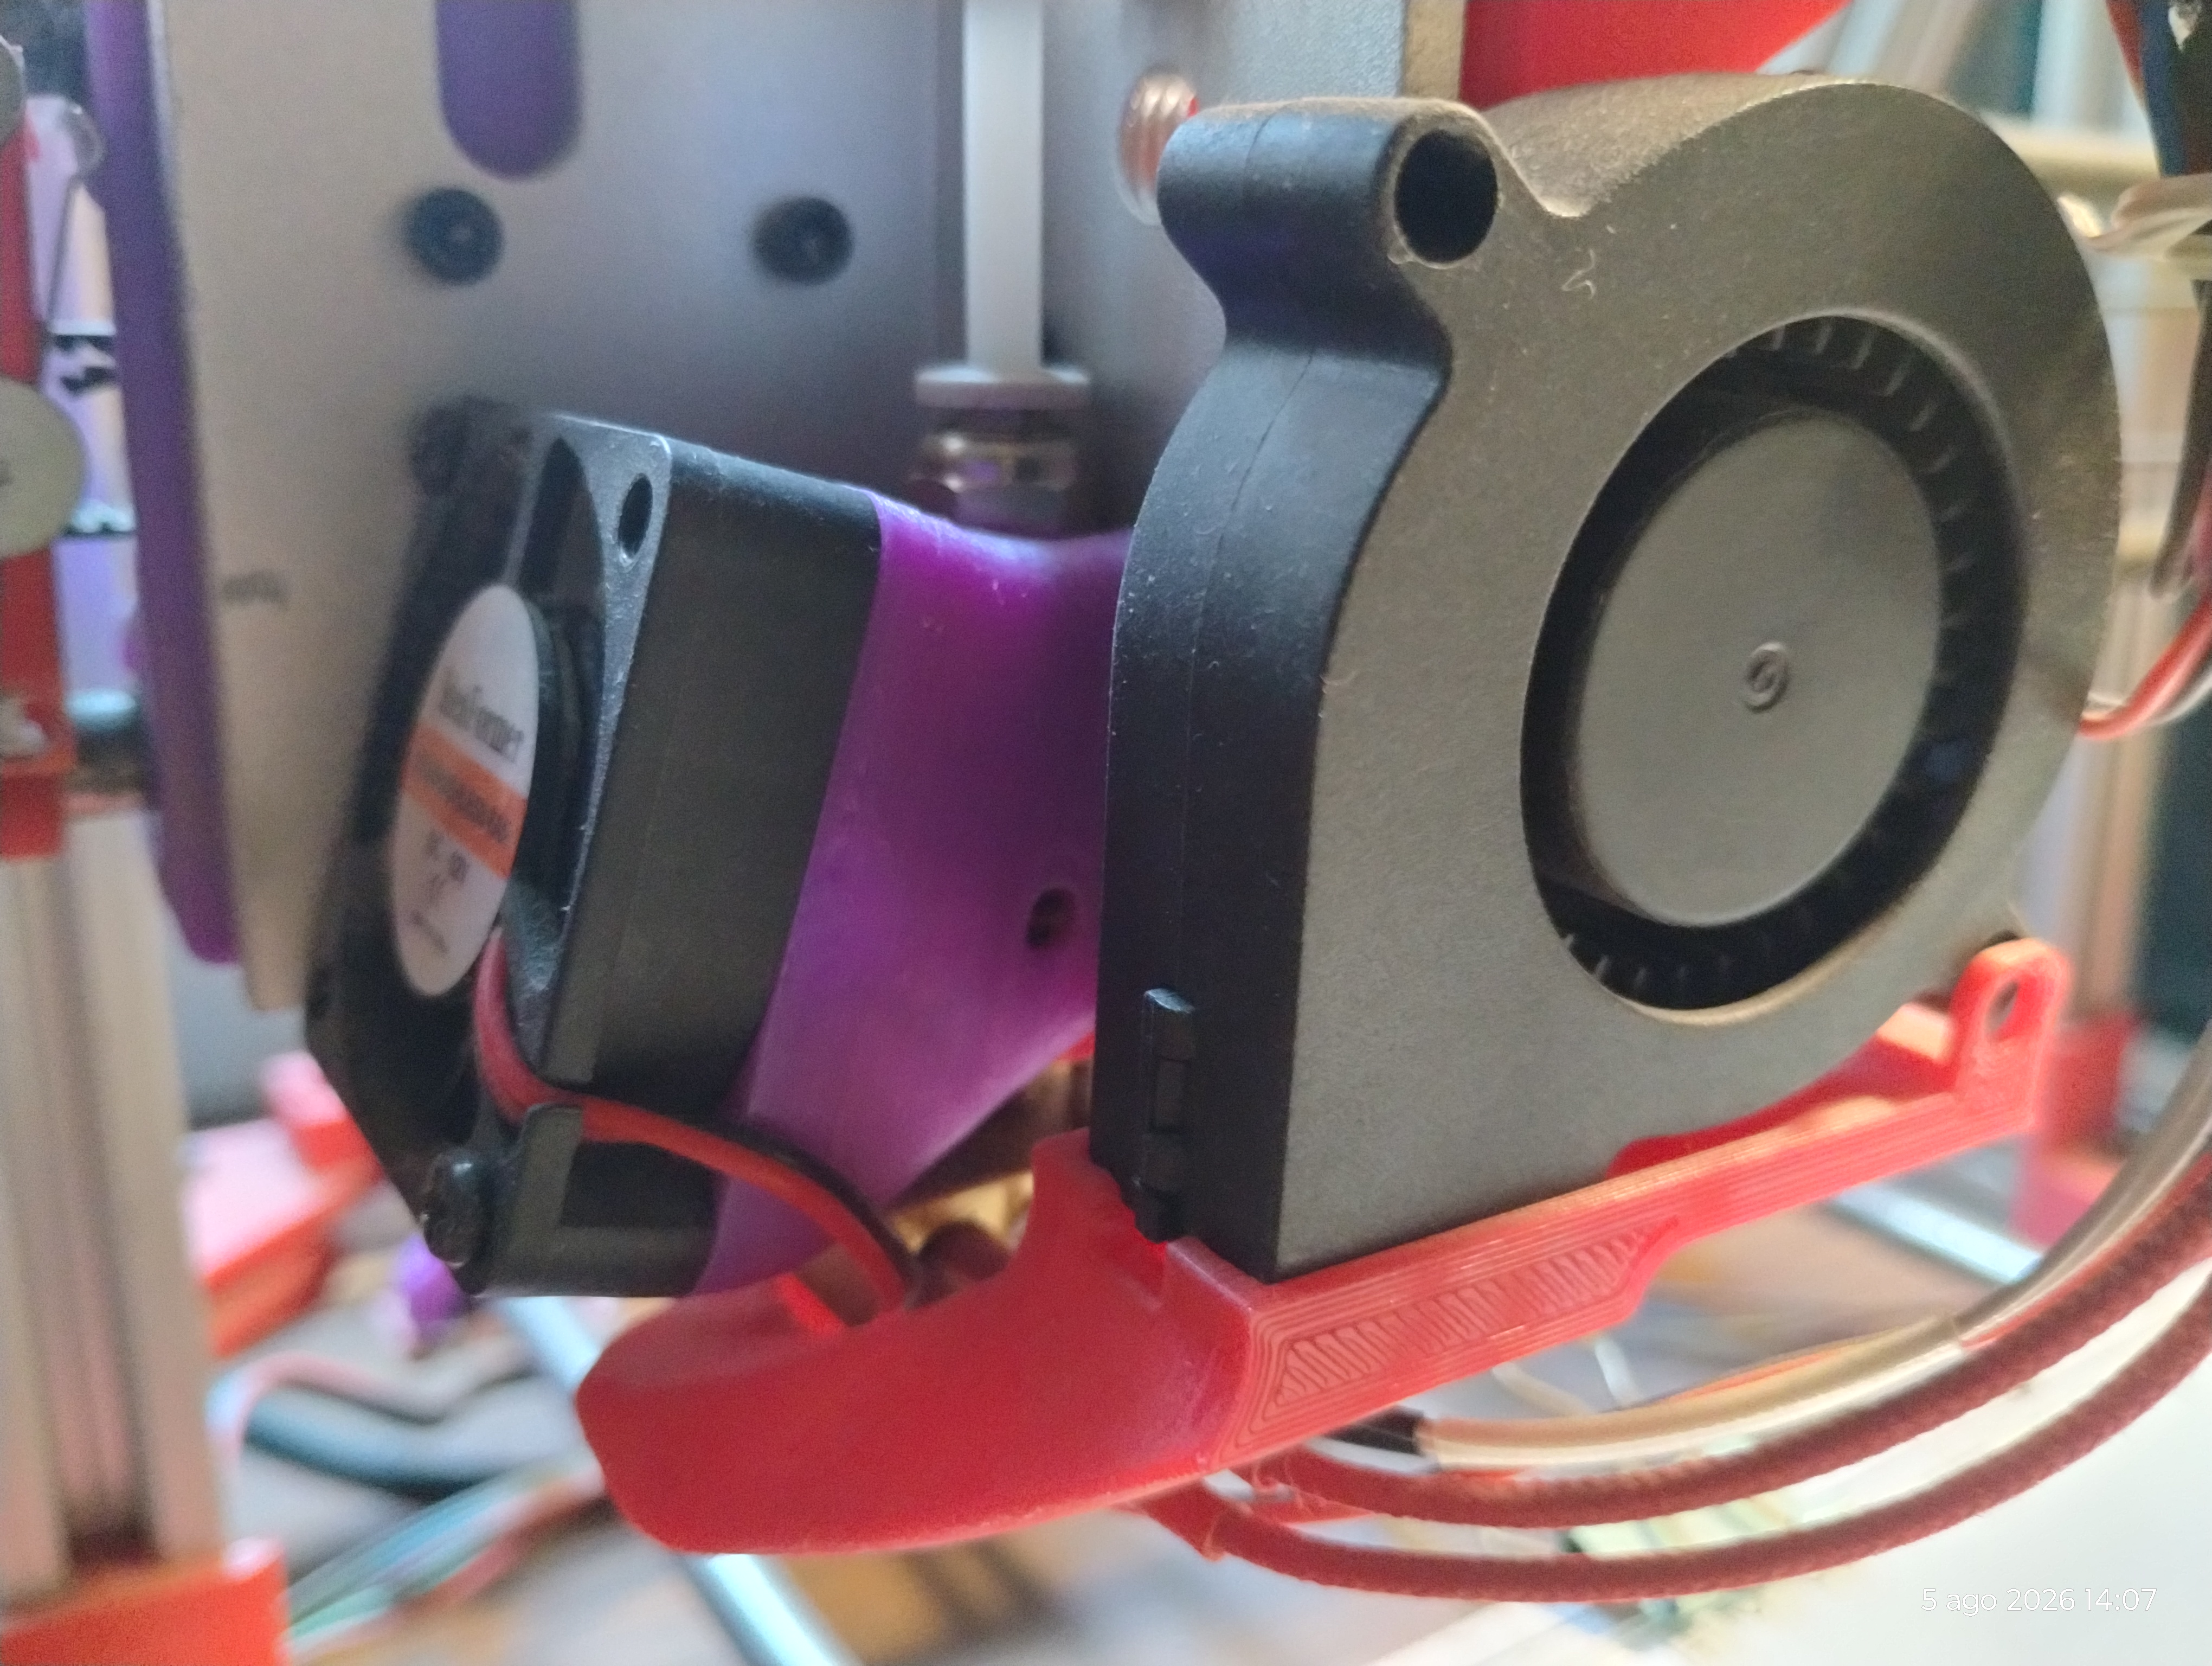
\includegraphics[width=0.5\linewidth]{ventiladores.jpg}
    \caption{Ventiladores}
    \label{fig:placeholder999}
\end{figure}
Funcionamiento correcto del ventilador del hotend y de capa.




\section{Parámetros finales de operación}

\begin{figure}[H]
    \centering
    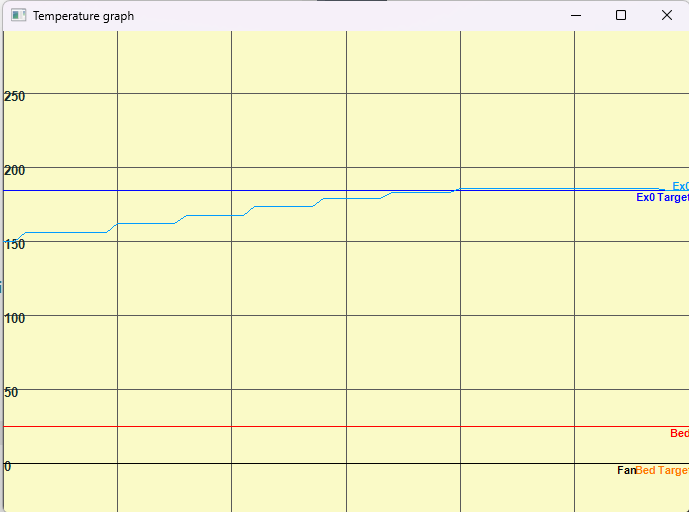
\includegraphics[width=0.5\linewidth]{Temperatura Hotend.png}
    \caption{Gráfica de temperatura}
    \label{fig:placeholder1000}
\end{figure}


Parámetros de impresión configurados

Temperatura, configuración automática/manual, tiempo, estabilidad.
Tabla con los valores definitivos: temperatura de extrusión, cama, altura de capa, velocidad, relleno, perímetros.
(tabla de parámetros Cura, constantes PID finales (Kp, Ki, Kd))

Am
Para


Calibración dimensional
Mediciones de cubos de calibración en los tres ejes (X, Y, Z). Error porcentual o absoluto respecto al modelo CAD.
(tabla de mediciones con vernier error promedio por eje)

\begin{figure}[H]
    \centering
    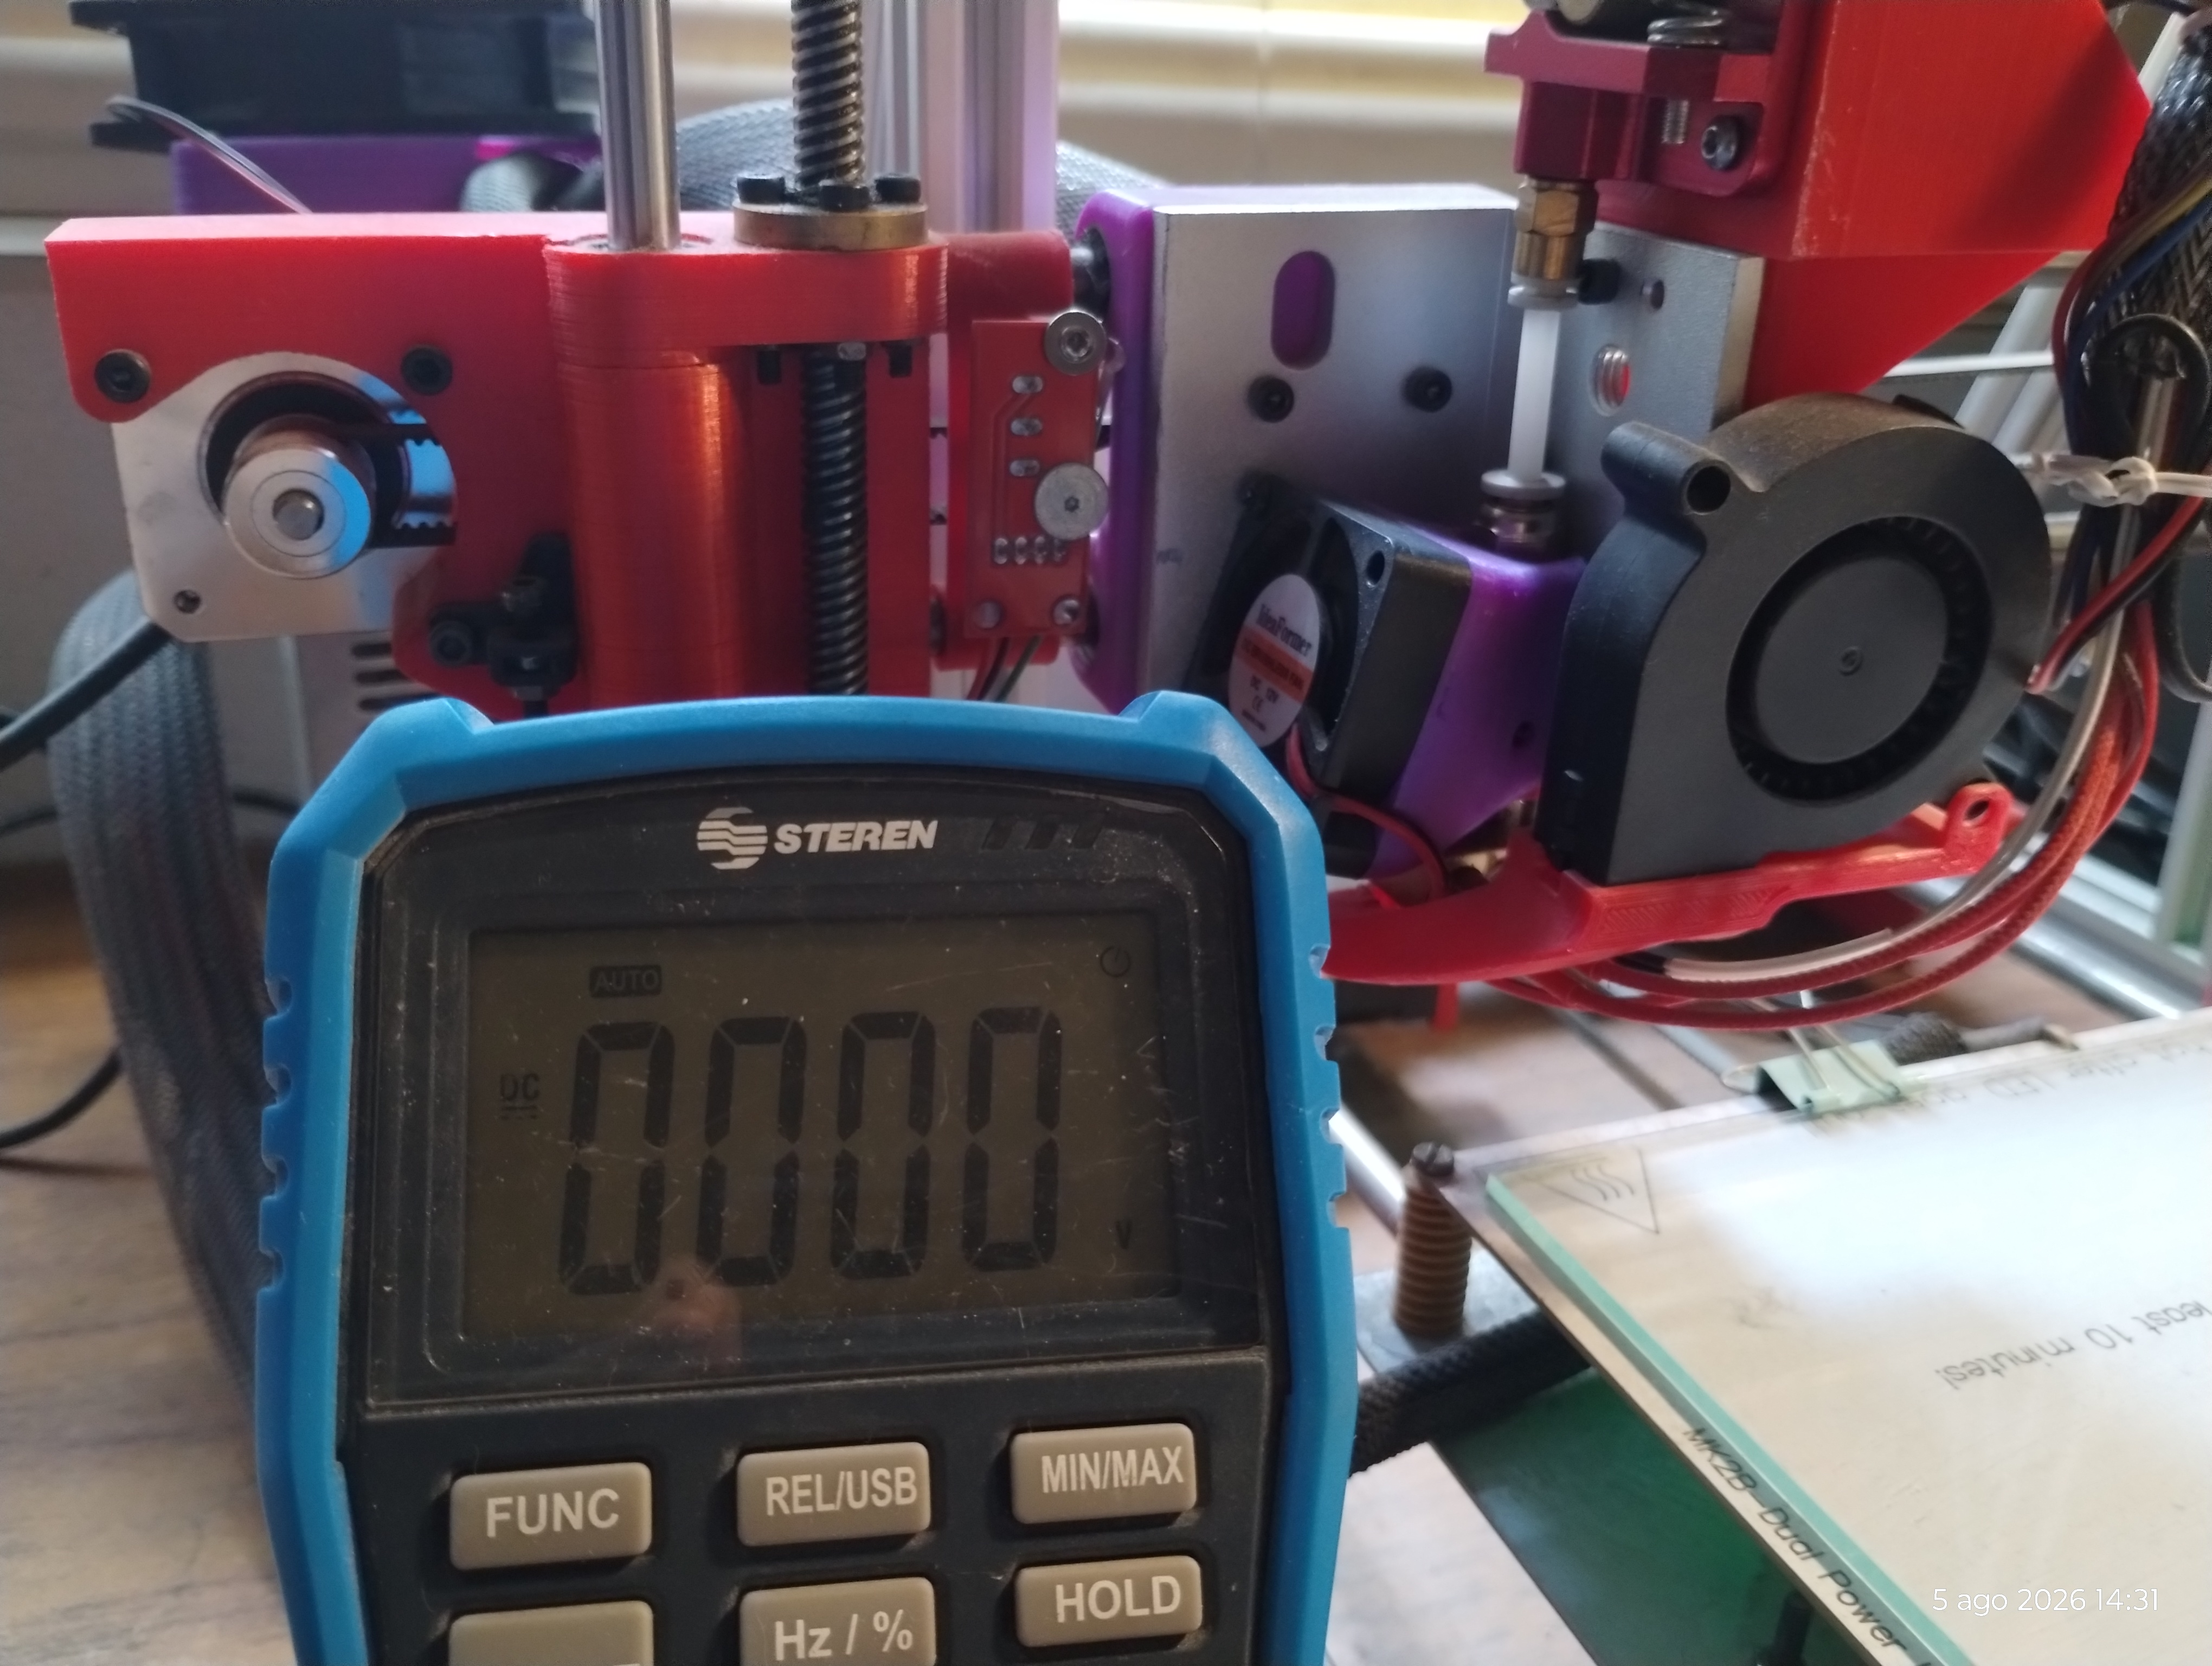
\includegraphics[width=0.5\linewidth]{evidencia hotend.jpg}
    \caption{Comporbacion temperatura del Hotend}
    \label{fig:placeholder1001}
\end{figure}
 \begin{figure}[H]
     \centering
     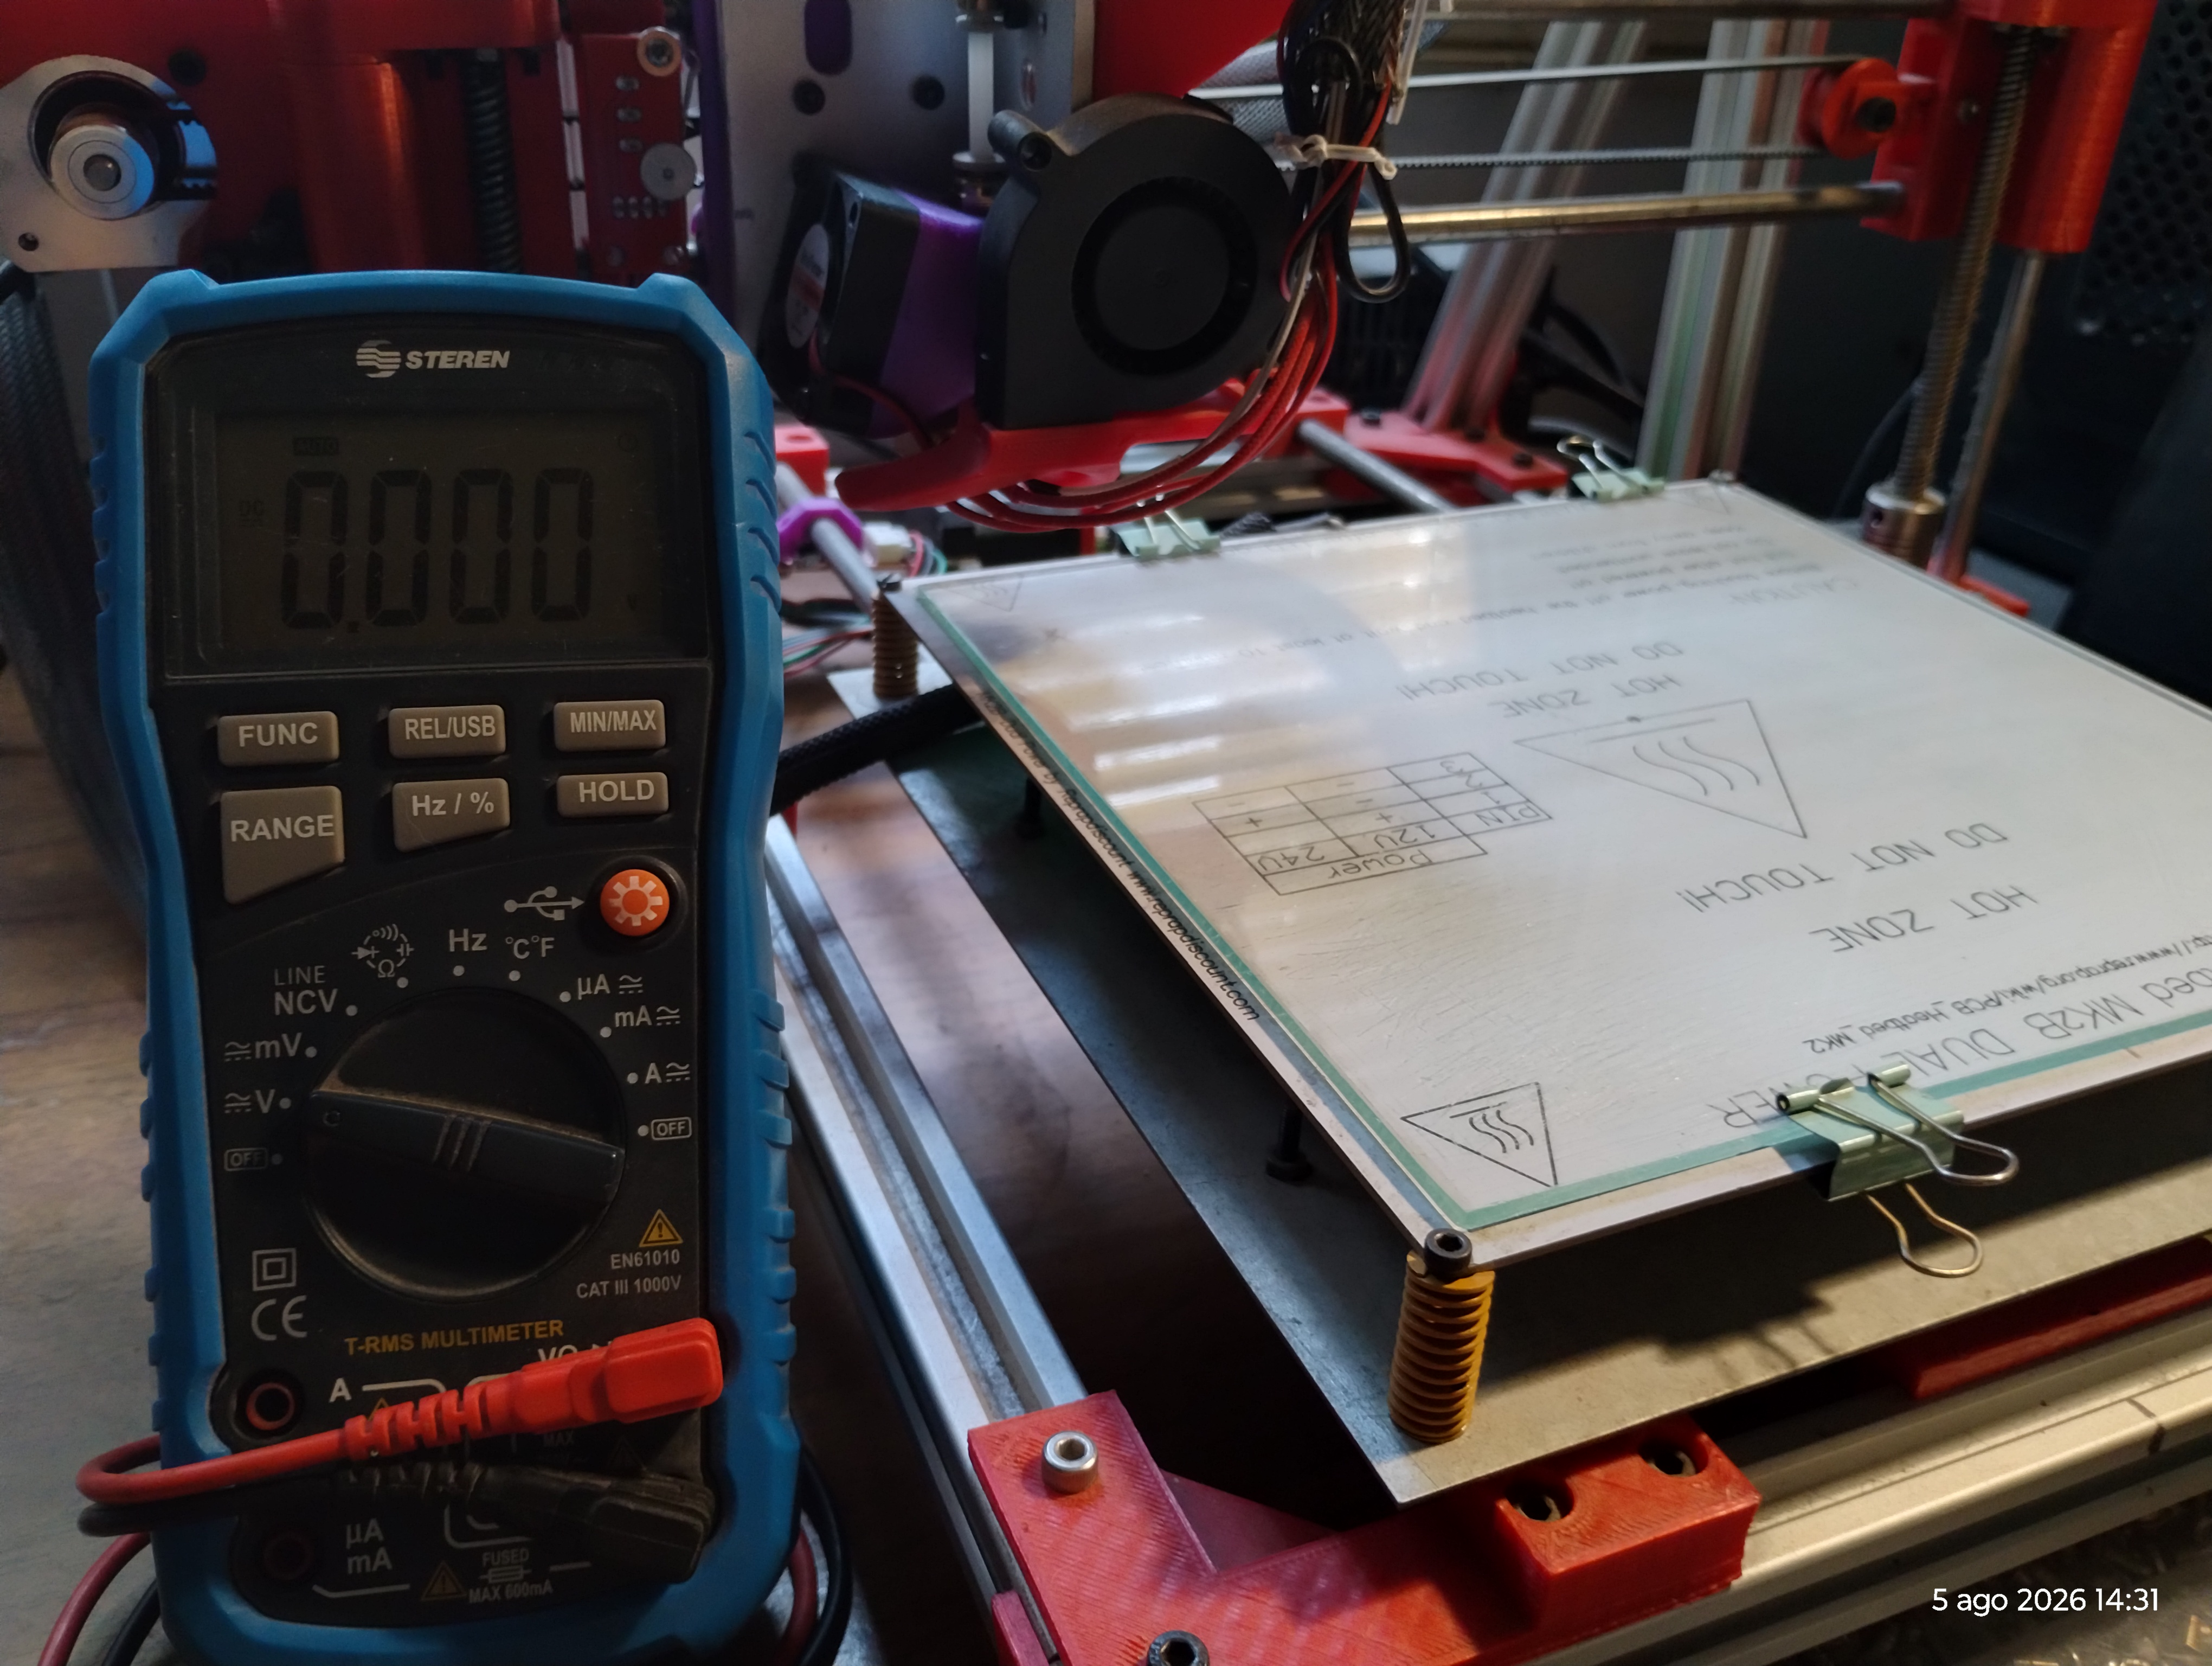
\includegraphics[width=0.5\linewidth]{evidencia cama.jpg}
     \caption{Comprobacion de temperatura de cama caleinte}
     \label{fig:placeholder1002}
 \end{figure}


\section{Evaluación de calidad de impresión}
\begin{figure}[H]
    \centering
    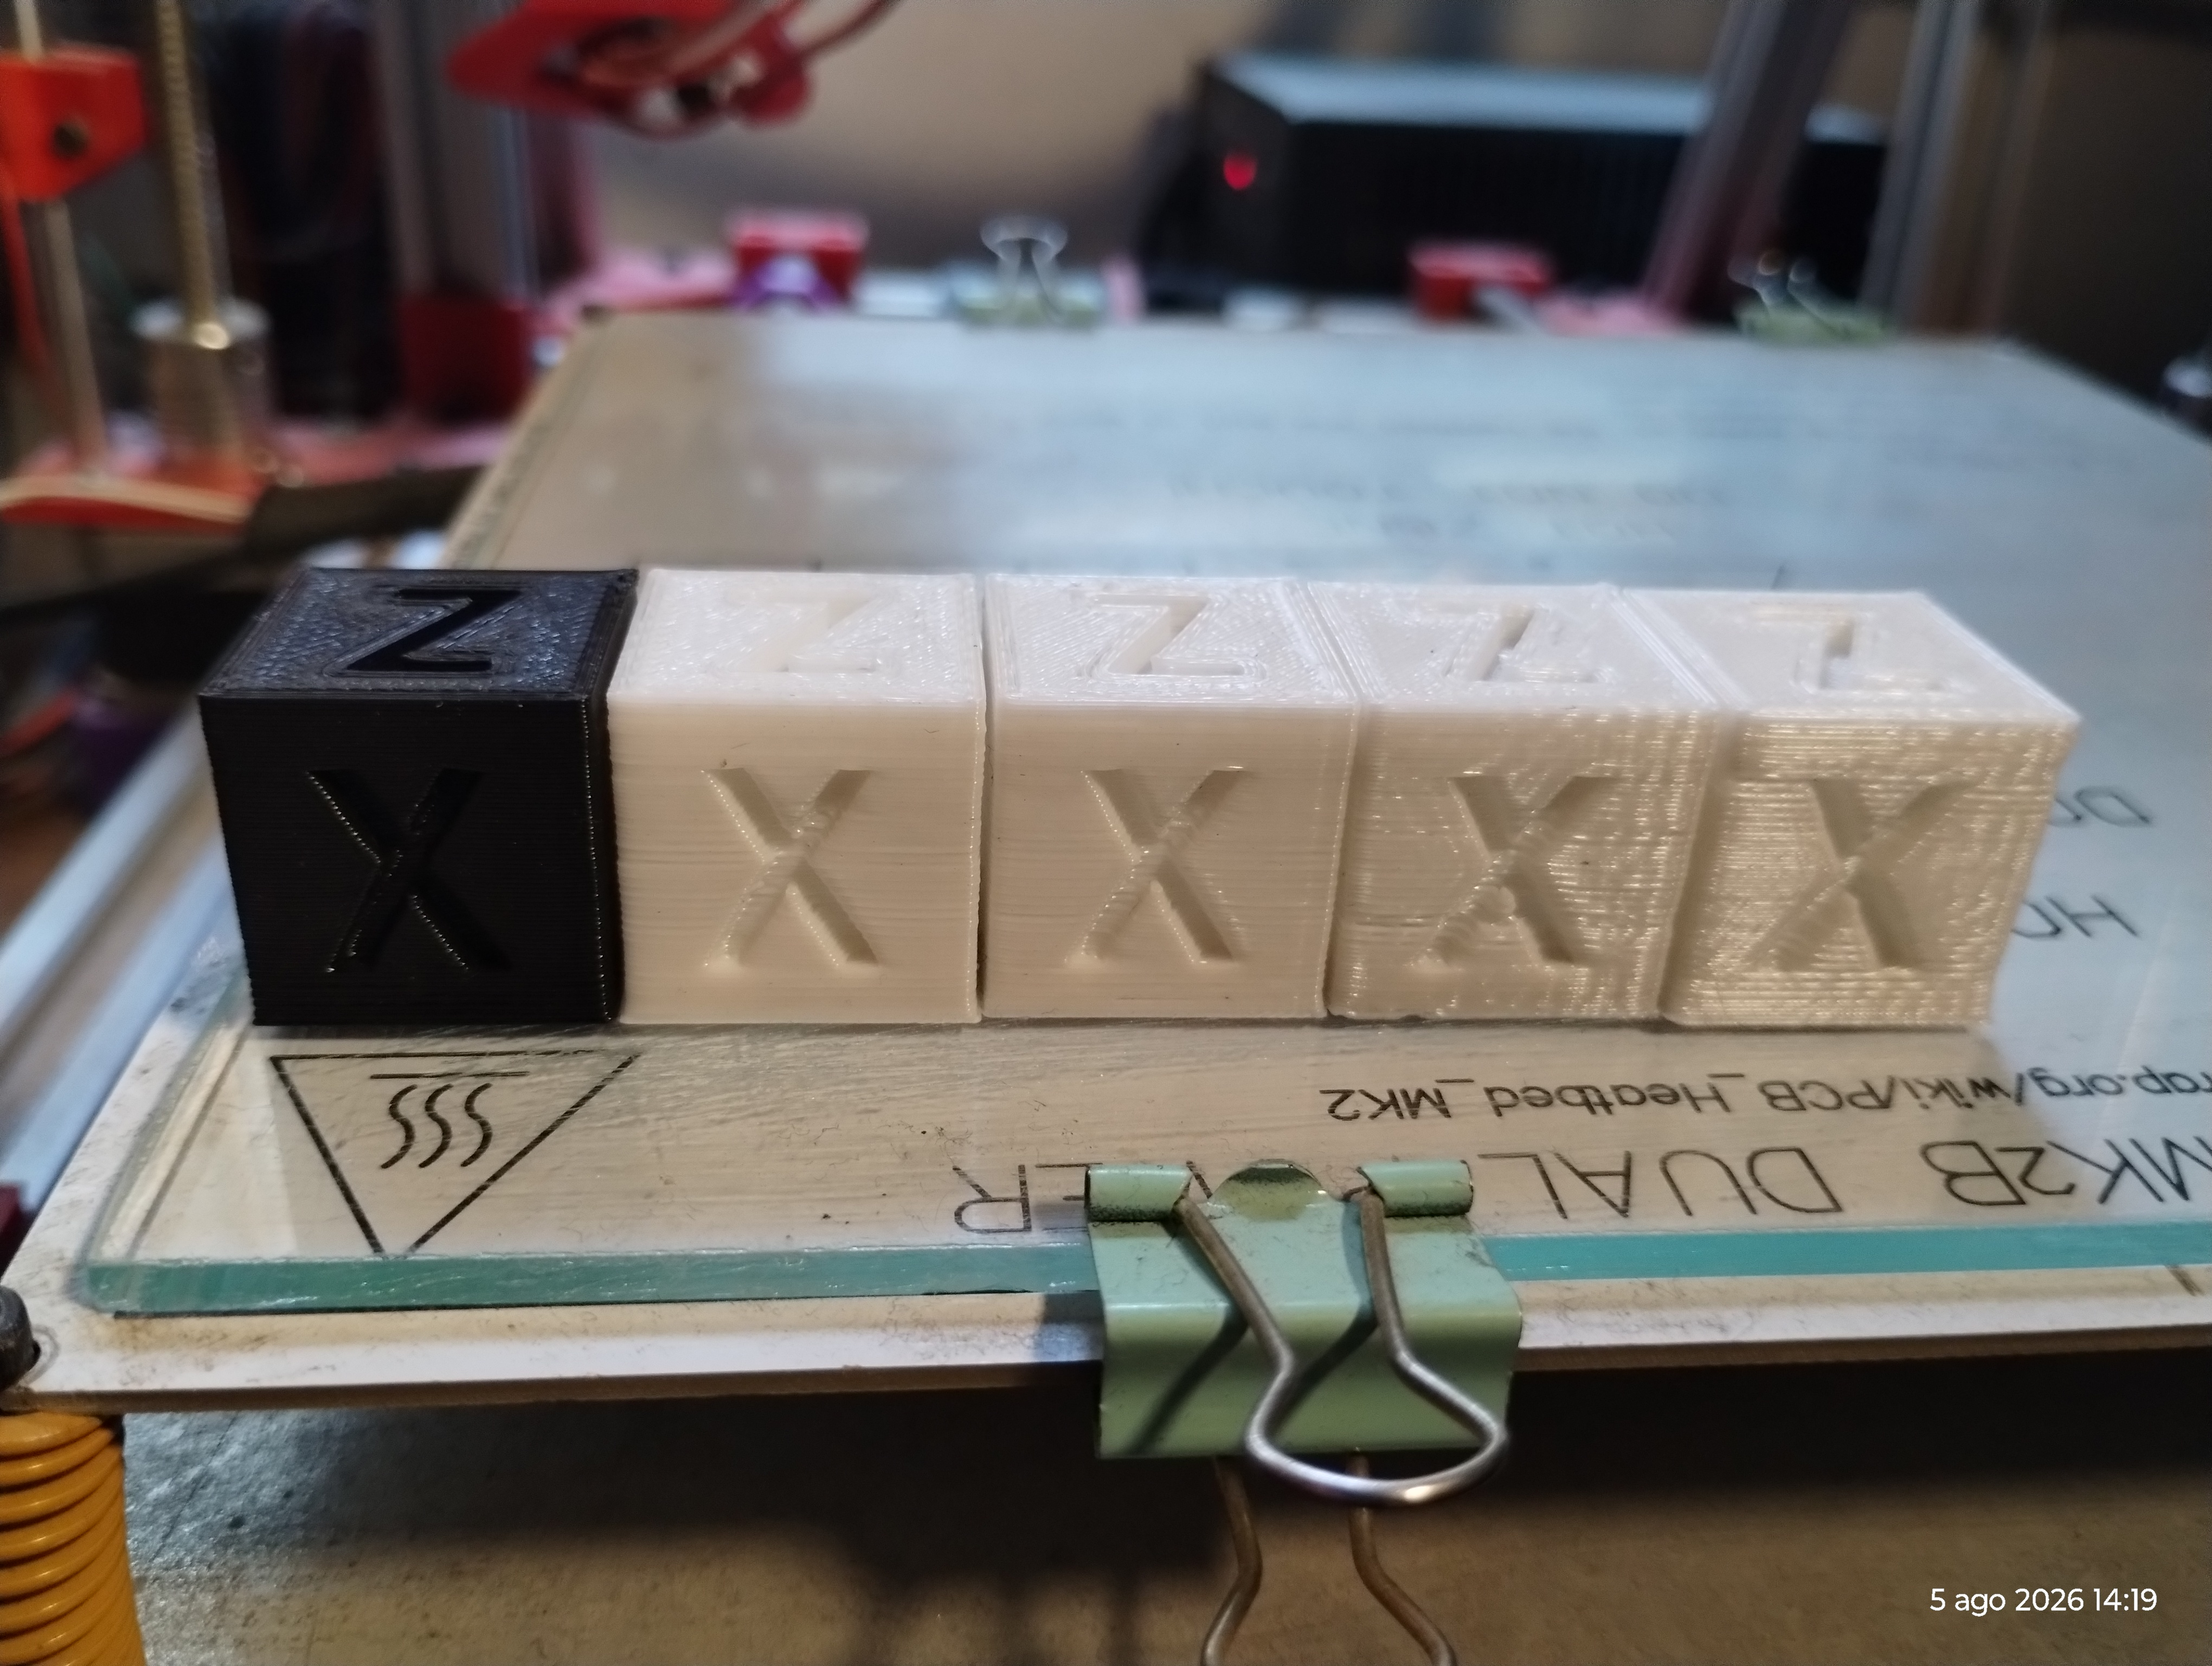
\includegraphics[width=0.5\linewidth]{cubos.jpg}
    \caption{Calidad de impresion}
    \label{fig:placeholder1003}
\end{figure}

\begin{figure}[H]
    \centering
    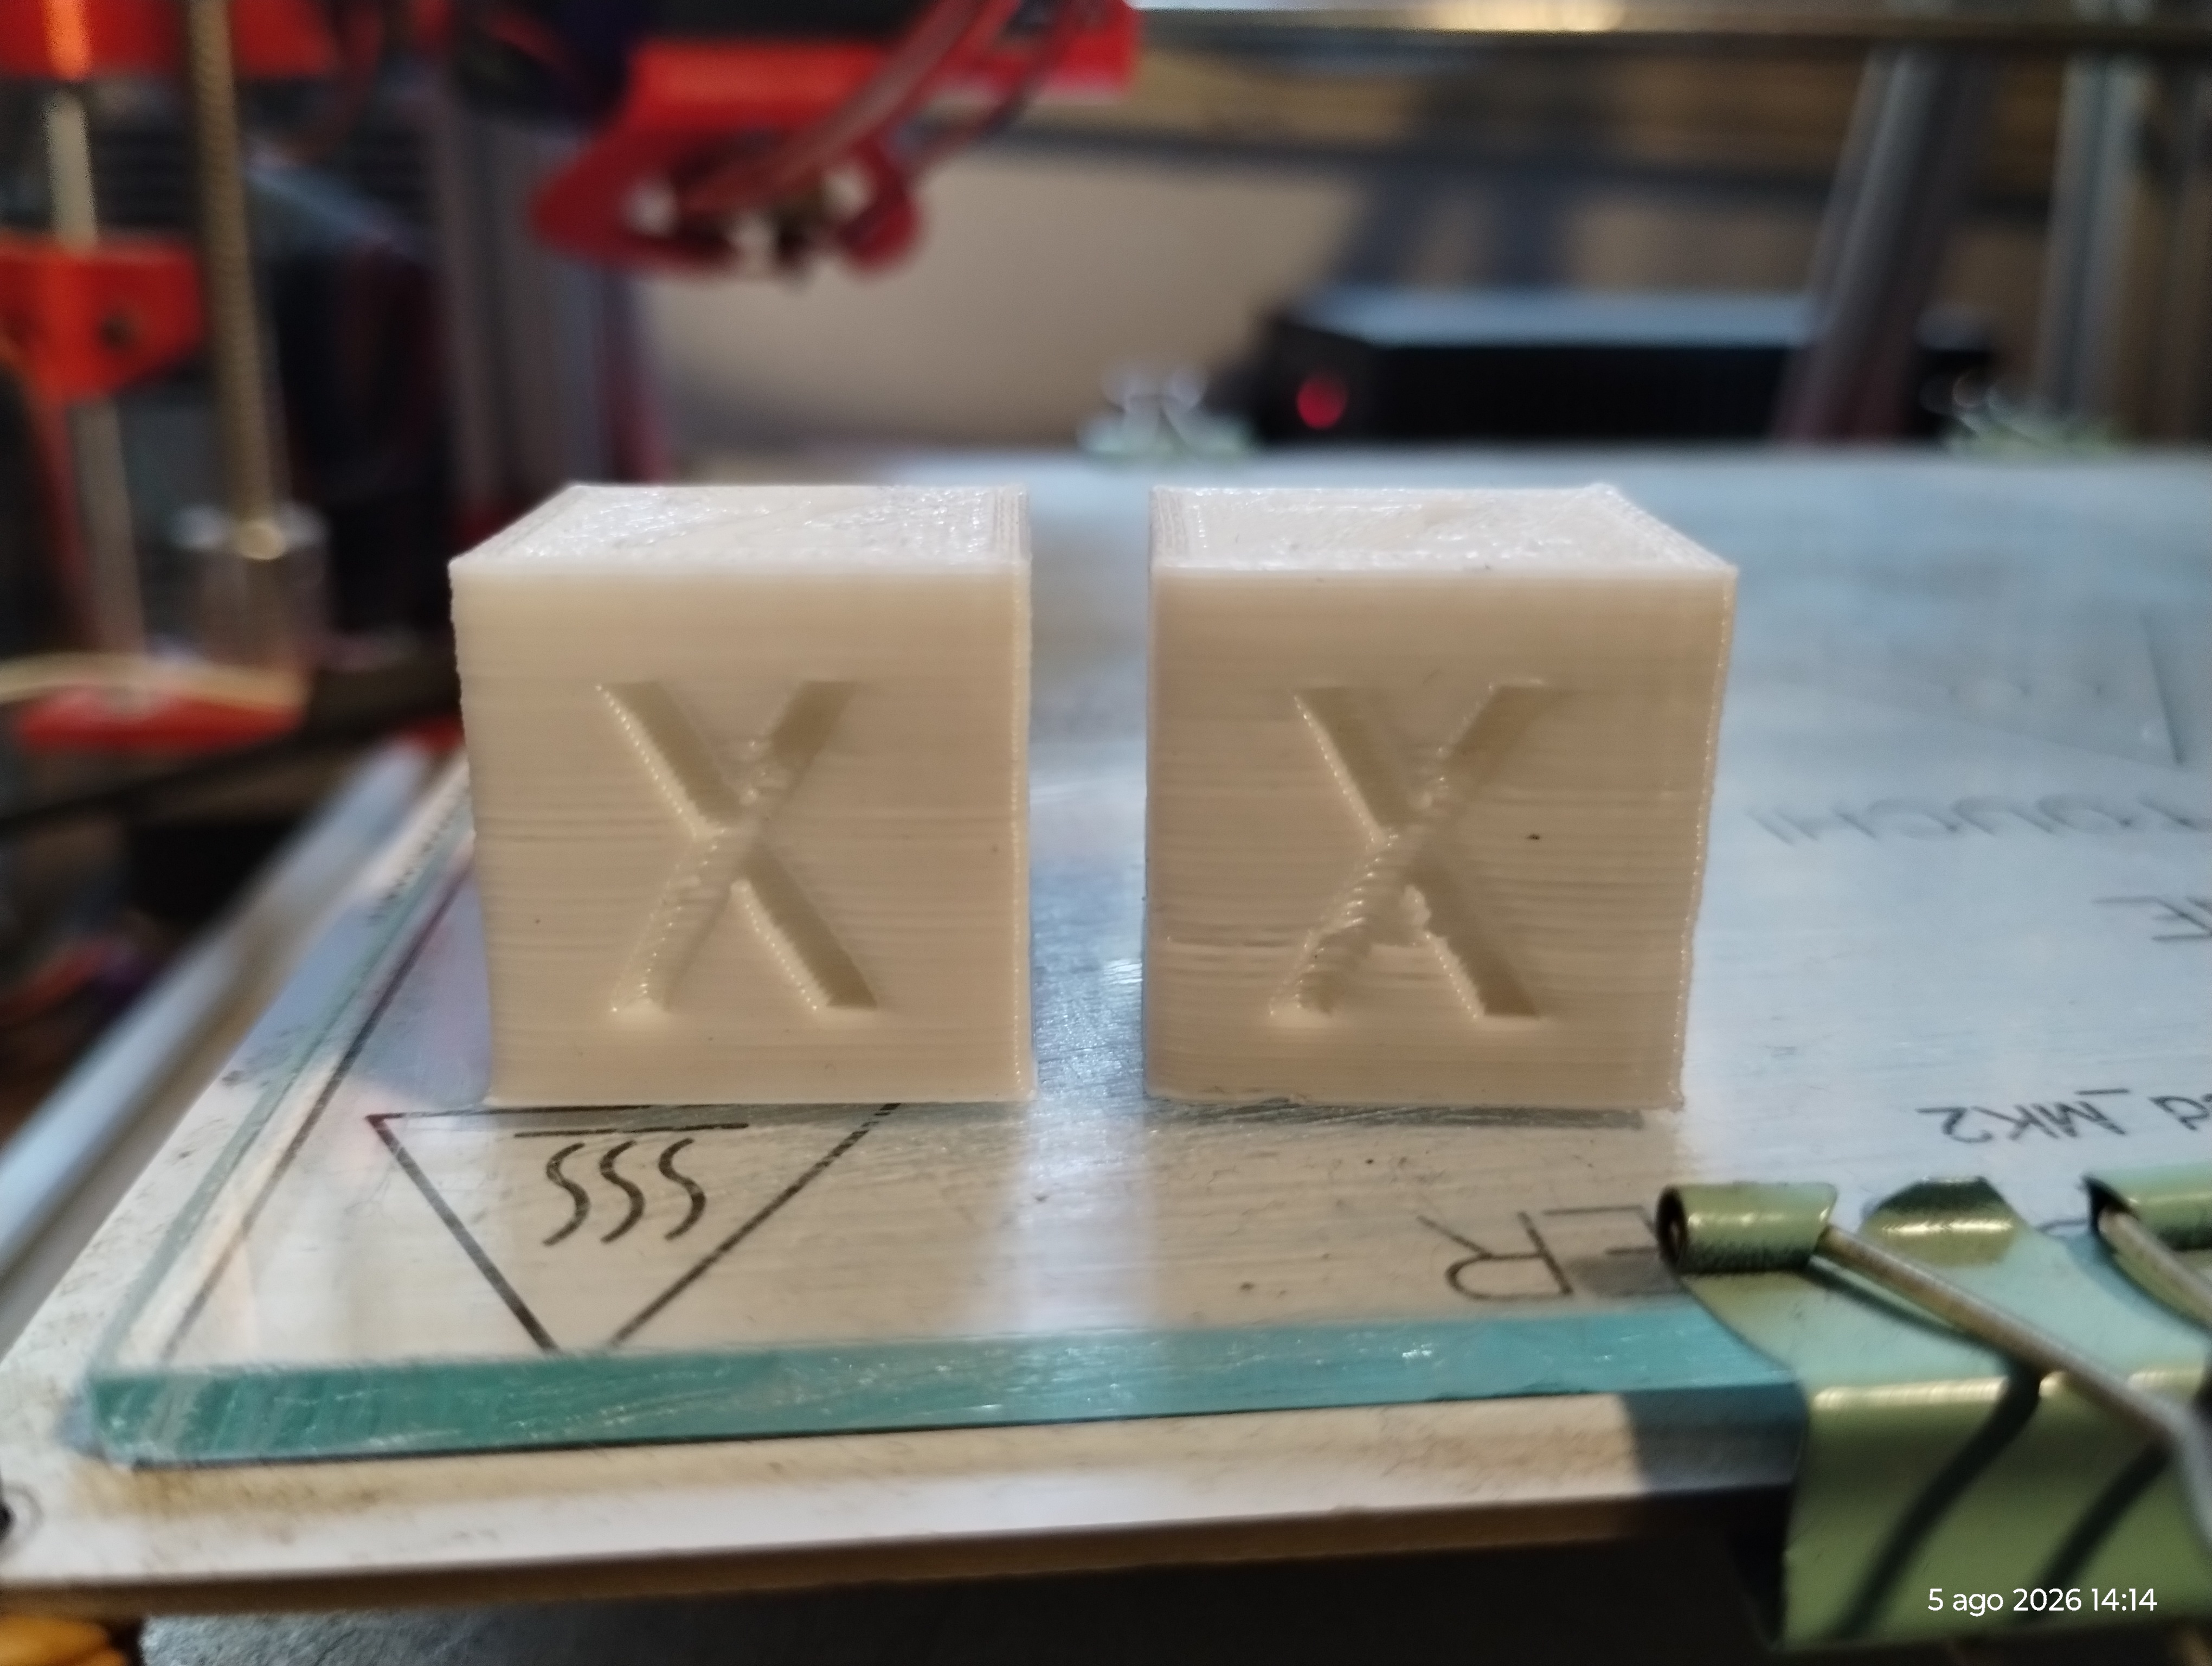
\includegraphics[width=0.5\linewidth]{comparacion calidad.jpg}
    \caption{Comparacion de piezas logradas}
    \label{fig:placeholder1004}
\end{figure}
\subsubsection{Evaluación de calidad superficial y defectos}
Resultados visuales de las pruebas de overhangs, bridges y repetibilidad. Presencia o ausencia de ghosting, stringing, warping.
fotos de piezas de prueba descripción objetiva de defectos observados

\section{Evaluación económica}
Análisis de costo
Tabla con desglose de costos del sistema construido vs. precio de mercado de una impresora comercial equivalente.
tabla comparativa de costo


%Probando el cambio en los codigos otra vez
%Hola Angel
%Te quiero guapo

%Ultima prueba de cambio en el archivo


